% ============================================================
%  Practica Experimental 4 (PE4) -- Unidad IV
%  Validacion, Gestion de Requisitos y Herramientas CASE
%  Asignatura: Ingenieria de Requerimientos [20303] -- UTEQ 2026-2027 PPA
%  Sistema del PFC: MundiPets -- Equipo D
%  Formato: IEEE onecolumn | Biber + biblatex (estilo IEEE)
% ============================================================

\documentclass[journal,onecolumn]{IEEEtran}

% ── Codificacion e idioma ───────────────────────────────────
\usepackage[T1]{fontenc}
\usepackage[utf8]{inputenc}
\usepackage[spanish, es-tabla]{babel}
\usepackage[autostyle=true, spanish=mexican]{csquotes}
\usepackage[htt]{hyphenat}

% ── Tablas ──────────────────────────────────────────────────
\usepackage{booktabs}
\usepackage{tabularx}
\usepackage{array}
\usepackage{multirow}
\usepackage{longtable}
\newcolumntype{C}[1]{>{\centering\arraybackslash}p{#1}}
\newcolumntype{L}[1]{>{\raggedright\arraybackslash}p{#1}}
\renewcommand{\thetable}{\arabic{table}}
\def\tablename{Tabla}

% ── Figuras ─────────────────────────────────────────────────
\usepackage{graphicx}
\graphicspath{{figuras/}{./}}
\usepackage{float}

% ── Color ───────────────────────────────────────────────────
\usepackage{xcolor}
\definecolor{uteqverde}{RGB}{0,110,60}

% ── Geometria ───────────────────────────────────────────────
\usepackage{geometry}
\geometry{a4paper, top=2.5cm, bottom=2.5cm, left=2.5cm, right=2.5cm,
	headheight=14pt, footskip=1.2cm}

% ── Encabezado y pie ────────────────────────────────────────
\usepackage{fancyhdr}
\pagestyle{fancy}
\fancyhf{}
\renewcommand{\headrulewidth}{0.4pt}
\fancyhead[L]{\small PE4 -- Unidad IV -- Ingeniería de Requerimientos}
\fancyhead[R]{\small MundiPets -- Equipo D}
\fancyfoot[C]{\thepage}

% ── Espaciado y listas ──────────────────────────────────────
\usepackage{parskip}
\setlength{\parskip}{4pt}
\makeatletter
\@ifundefined{labelindent}{}{\let\labelindent\relax}
\makeatother
\usepackage{enumitem}
\usepackage{amssymb}
\usepackage{amsmath}

% ── Titulos de seccion ──────────────────────────────────────
\usepackage{titlesec}
\renewcommand{\thesection}{\arabic{section}}
\renewcommand{\thesubsection}{\thesection.\arabic{subsection}}
\renewcommand{\thesubsubsection}{\thesubsection.\arabic{subsubsection}}
\titleformat{\section}{\normalfont\Large\bfseries}{\thesection}{1em}{}
\titleformat{\subsection}{\normalfont\large\bfseries}{\thesubsection}{1em}{}
\titleformat{\subsubsection}{\normalfont\normalsize\bfseries}{\thesubsubsection}{1em}{}
\setcounter{secnumdepth}{4}
\setcounter{tocdepth}{4}

% ── Leyendas ────────────────────────────────────────────────
\usepackage{caption}
\captionsetup{font=small, labelfont=bf}

% ── Codigo / listados (capturas de comandos git, CSV, etc.) ─
\usepackage{listings}
\definecolor{codegray}{gray}{0.95}
\lstdefinestyle{consola}{
	backgroundcolor=\color{codegray},
	basicstyle=\ttfamily\footnotesize,
	showstringspaces=false,
	breaklines=true,
	frame=single,
	rulecolor=\color{gray!50},
	tabsize=2,
	captionpos=b
}
\lstset{style=consola}
\lstset{literate=%
	{á}{{\'a}}1 {é}{{\'e}}1 {í}{{\'i}}1 {ó}{{\'o}}1 {ú}{{\'u}}1
	{Á}{{\'A}}1 {É}{{\'E}}1 {Í}{{\'I}}1 {Ó}{{\'O}}1 {Ú}{{\'U}}1
	{ñ}{{\~n}}1 {Ñ}{{\~N}}1 {ü}{{\"u}}1
}
\renewcommand{\lstlistingname}{Código}

% ── Bibliografia (biber + estilo IEEE) ──────────────────────
\usepackage[
backend=biber,
style=ieee,
citestyle=numeric-comp,
isbn=true,
doi=true
]{biblatex}
\addbibresource{referencias.bib}

% ── Enlaces ─────────────────────────────────────────────────
\usepackage[hidelinks,colorlinks=false]{hyperref}

% ============================================================
%  ENTORNO REUTILIZABLE PARA FORMULARIOS (RFC, Anexo A, etc.)
% ============================================================
\newenvironment{atributos}[2]{%
	\small
	\begin{longtable}{@{}>{\raggedright\arraybackslash}p{4.2cm} >{\raggedright\arraybackslash}p{11.2cm}@{}}
		\caption{#2}\label{tab:#1}\\
		\toprule
		\textbf{Campo} & \textbf{Contenido} \\
		\midrule
		\endfirsthead
		\multicolumn{2}{@{}l}{\small\itshape (continuación)}\\
		\toprule
		\textbf{Campo} & \textbf{Contenido} \\
		\midrule
		\endhead
		\bottomrule
		\endlastfoot
	}{%
	\end{longtable}
	\normalsize
}

% ============================================================
\begin{document}
	
	% ========================================================
	% 1. CARÁTULA
	% ========================================================
	\begin{titlepage}
		\centering
		
		{\large\bfseries UNIVERSIDAD TÉCNICA ESTATAL DE QUEVEDO\\[12pt]}
		
		
\includegraphics[width=0.2\textwidth]{figuras/logo_uteq.png}\\[12pt]
		
		{\large\bfseries FACULTAD DE CIENCIAS DE LA COMPUTACIÓN\\[4pt]
			CARRERA DE INGENIERÍA EN SOFTWARE}
		
		\vspace{0.3cm}
		
		{\normalsize\bfseries TEMA:}\\[4pt]
		{\normalsize PRÁCTICA EXPERIMENTAL -- UNIDAD IV\\
			VALIDACIÓN, GESTIÓN DE REQUISITOS Y HERRAMIENTAS CASE}\\[4pt]
		
		\vspace{0.2cm}
		
		{\normalsize\bfseries MATERIA:}\\[4pt]
		{\normalsize INGENIERÍA DE REQUERIMIENTOS}
		
		\vspace{0.2cm}
		
		{\normalsize\bfseries DOCENTE:}\\[4pt]
		{\normalsize ING. GUERRERO ULLOA GLEISTON CICERÓN, PhD.}
		
		\vspace{0.2cm}
		
		{\normalsize\bfseries INTEGRANTES (EQUIPO D):}\\[6pt]
		
		\textit{\textbf{MORALES SÁNCHEZ GARY ALEJANDRO}},~CI: 1251154173,~gmoraless2@uteq.edu.ec\\
		{\small Rol en la práctica: Moderador}\\[6pt]
		
		\textit{SÁNCHEZ CORNEJO GARY ALBERTO},~CI: 1208338291,~gsanchezc6@uteq.edu.ec\\
		{\small Rol en la práctica: Lector + Inspector 1}\\[6pt]
		
		\textit{CEDEÑO CORONADO WILSON LIZANDRO},~CI: 1206867200,~wcedenoc2@uteq.edu.ec\\
		{\small Rol en la práctica: Inspector 2}
		
		\vspace{0.2cm}
		
		{\normalsize\bfseries SISTEMA DEL PFC:}\\[4pt]
		{\normalsize MundiPets --- Plataforma para el cruce y la adopción responsable de mascotas}
		
		\vspace{0.2cm}
		
		{\normalsize\bfseries CURSO:}\\[4pt]
		{\normalsize CUARTO SEMESTRE PARALELO \enquote{B}}
		
		\vspace{0.2cm}
		
		\textbf{Repositorio GitHub (ISR401-PFC-ERS-EquipoD):}\\
		\url{https://github.com/gsanchezc6-beep/ISR401-PFC-ERS-EquipoD}
		
		\vspace{1.0cm}
		
		{\normalsize\bfseries QUEVEDO -- LOS RÍOS -- ECUADOR}\\[4pt]
		{\normalsize\bfseries 2026 -- 2027 PPA}
		
	\end{titlepage}
	
	\newpage
	\tableofcontents
	\newpage
	\listoftables
	\newpage
	
	% La Sección 1 de la Guía y Rúbrica PE4 es la Carátula (no
	% numerada como sección de \LaTeX{}, ya cubierta arriba); el
	% contador se adelanta para que "Resumen y objetivos" sea la
	% Sección 2, conforme a la estructura obligatoria del informe.
	
	% ========================================================
	% 2. RESUMEN Y OBJETIVOS
	% ========================================================
	\section{Resumen y objetivos}
	\label{sec:resumen}
	
	\subsection{Resumen}
	
	Este informe documenta la aplicación de técnicas formales de
	validación y gestión de requisitos sobre la Especificación de
	Requisitos de Software (ERS) del proyecto MundiPets, plataforma
	para el cruce y la adopción responsable de mascotas, en su versión
	1.0 de 147 páginas. Se ejecutó una inspección formal según el
	método Fagan con roles diferenciados, preparación individual
	acreditada mediante control de versiones y una reunión de
	consolidación de 92 minutos, de la que resultaron 18 defectos
	únicos clasificados por tipo y severidad sobre las seis propiedades
	de calidad de ISO/IEC/IEEE 29148:2018. Se calcularon cinco métricas
	de inspección y se interpretó cada una respecto del estado real del
	documento. A partir de los defectos detectados se tramitaron tres
	solicitudes formales de cambio de naturaleza distinta (alcance,
	calidad y normativa), cuyo análisis de impacto se derivó recorriendo
	la matriz de trazabilidad extendida del propio ERS. Un \emph{Change
		Control Board} simulado deliberó y decidió sobre cada solicitud,
	dando origen a la versión 1.1 del documento. La trazabilidad se
	implementó en una herramienta CASE y la línea base se publicó
	mediante etiqueta anotada en un repositorio Git público.
	
	\subsection{Objetivo general}
	
	Aplicar técnicas formales de validación de requisitos, gestionar
	cambios mediante un \emph{Change Control Board} simulado,
	implementar la trazabilidad en una herramienta CASE y establecer una
	línea base con Git sobre el ERS real del Proyecto Fin de Curso
	MundiPets.
	
	\subsection{Objetivos específicos}
	
	\begin{enumerate}[label=\arabic*.]
		\item Ejecutar una inspección formal tipo Fagan sobre el ERS del
		PFC, con roles diferenciados, lista de verificación y registro
		de defectos.
		\item Calcular e interpretar métricas de inspección (densidad
		de defectos, distribución por tipo y severidad, tasa de
		corrección).
		\item Tramitar tres solicitudes formales de cambio (RFC) con
		análisis de impacto sustentado en la matriz de trazabilidad.
		\item Deliberar y decidir en un CCB simulado, dejando acta
		motivada y versión actualizada del ERS.
		\item Construir la trazabilidad bidireccional del ERS en una
		herramienta CASE de gestión con campos personalizados y
		enlaces verificables.
		\item Establecer y publicar la línea base del ERS con control
		de versiones (\emph{commit} semántico, \emph{tag} anotado y
		\texttt{CHANGELOG.md}).
		\item Comparar herramientas CASE de IR y contrastar IR
		tradicional frente a IR ágil, cerrando con conclusiones
		críticas propias.
	\end{enumerate}
	
	% ========================================================
	% 3. FUNDAMENTO TEÓRICO
	% ========================================================
	\section{Fundamento teórico}
	\label{sec:fundamento}
	
	\subsection{Marco normativo aplicado a la validación y gestión de requisitos}
	\label{sec:marco-normativo}
	
	\subsubsection{Validación de requisitos según IEEE/ISO/IEC 29148}
	
	La norma IEEE/ISO/IEC~29148:2018~\cite{ieee29148_2018} es el estándar
	de referencia para los procesos de Ingeniería de Requisitos y, en
	particular, en su sección 6.4 (\emph{Software Requirements
		Validation Process}) define la validación como la comprobación de
	que el conjunto de requisitos especificados es correcto, completo,
	consistente y trazable con respecto a las necesidades del
	interesado, y de que cada requisito individual satisface un
	conjunto de atributos de calidad. Estos atributos --- no
	ambigüedad, completitud, consistencia, verificabilidad,
	trazabilidad y factibilidad --- constituyen el criterio operativo
	con el que se diseñó la Lista de Verificación de Inspección
	(Anexo~A) empleada en la Sección~\ref{sec:fagan} de este informe, y
	son precisamente los seis ejes bajo los cuales el equipo clasificó
	cada defecto detectado en el ERS de MundiPets.
	
	La norma distingue explícitamente la validación de la
	verificación: mientras la verificación comprueba que un artefacto
	cumple una especificación previa (¿se construyó correctamente el
	documento?), la validación comprueba que la especificación misma
	responde a la necesidad real del interesado (¿se especificó el
	documento correcto?)~\cite{ieee29148_2018}. Esta distinción es
	relevante para el caso de MundiPets: por ejemplo, el requisito
	RNF-02 fue calificado como defecto de verificabilidad porque su
	criterio (``monitorear la disponibilidad del sistema durante un mes
	de operación'') no puede ejecutarse dentro del ciclo de vida de un
	Proyecto de Fin de Curso que no contempla una fase de operación
	real: el requisito puede estar bien especificado conceptualmente,
	pero su criterio de aceptación no es válido para el contexto del
	proyecto.
	
	Pohl (2025)~\cite{pohl2025}, en la Parte V de su obra, complementa
	la norma señalando que la validación no debe entenderse como una
	actividad puntual al cierre del documento, sino como un conjunto
	de técnicas --- revisiones, inspecciones, prototipado y pruebas de
	aceptación tempranas --- que se aplican de forma incremental sobre
	cada versión del conjunto de requisitos. El SWEBOK
	v4.0~\cite{swebok2024}, secciones 1.6--1.8, coincide en ubicar la
	validación como un proceso continuo del ciclo de vida de requisitos
	y no como un evento aislado.
	
	\subsubsection{Inspecciones formales: el método Fagan}
	
	La técnica de inspección formal empleada en el Paso~1 de esta
	práctica (roles de Moderador, Lector e Inspectores; preparación
	individual; reunión de inspección; registro de defectos) proviene
	del trabajo seminal de Fagan (1976)~\cite{fagan1976}, quien
	demostró que la detección temprana de defectos mediante revisión
	estructurada por pares reduce significativamente el costo de
	corrección respecto a detectarlos en etapas posteriores del
	desarrollo. El método de Fagan introduce dos elementos que el
	equipo aplicó directamente: (a) la preparación individual
	obligatoria antes de la reunión, que evita que la revisión dependa
	de la lectura colectiva superficial de un solo participante, y (b)
	el registro cuantitativo de defectos por tipo y severidad, que
	permite calcular una densidad de defectos (defectos por página)
	como indicador objetivo de la madurez del documento inspeccionado.
	
	En la inspección del ERS de MundiPets, la aplicación independiente
	del Anexo~A por cada inspector --- Morales sobre la Sección 1-2,
	Sánchez sobre la Sección 3.2 y casos de uso, y Cedeño sobre la
	Sección 3.3, 3.4 y apéndices --- siguió este principio, evitando
	que un defecto real, como la contradicción de identidad del
	participante en la fila EV-04 del Apéndice B.3 (declarado
	simultáneamente como VET-02 y VET-04), pasara inadvertido por
	depender de la lectura de un único revisor.
	
	\subsubsection{Gestión del cambio y control de configuración}
	
	La gestión de cambios que se simula en el Paso~2 de esta práctica
	(Comité de Control de Cambios o CCB) tiene su fundamento normativo
	en IEEE/ISO/IEC~15288:2023~\cite{ieee15288_2023}, que define el
	proceso de gestión de la configuración como responsable de
	establecer líneas base (\emph{baselines}) y controlar las
	modificaciones sobre ellas, y en
	IEEE/ISO/IEC~12207:2017~\cite{ieee12207_2017}, que detalla el
	proceso de control de cambios específicamente para artefactos de
	software. El PMBOK, 7.\textsuperscript{a}~ed.~\cite{pmi2021}, por
	su parte, formaliza el CCB como el órgano formal responsable de
	aprobar, rechazar o diferir las solicitudes de cambio (RFC) dentro
	del sistema de control de cambios integrado de un proyecto,
	evaluando cada solicitud en función de su impacto en alcance,
	costo y cronograma. Este es el marco que sustenta el Formulario RFC
	(Anexo~C) y el Acta del CCB elaborados en la
	Sección~\ref{sec:ccb} de este informe.
	
	La calidad del documento resultante de este proceso --- el ERS en
	su versión 1.1 --- se evalúa con el modelo ISO/IEC~25010:2023
	(SQuaRE)~\cite{iso25010_2023}, que reemplaza al modelo de 2011 e
	introduce cambios estructurales relevantes: por ejemplo,
	Portabilidad deja de ser una característica de calidad de primer
	nivel y pasa a ser subcaracterística de Flexibilidad, y se
	incorpora Inocuidad (\emph{Safety}) como característica
	independiente. Precisamente por esta razón, uno de los defectos
	detectados en el ERS de MundiPets --- la tabla de cobertura de
	calidad del documento, que afirma cubrir ``las nueve
	características'' de ISO/IEC 25010:2023 pero mantiene la estructura
	de la versión 2011 --- constituye un ejemplo directo de
	desalineación con el estándar vigente citado por el propio
	documento.
	
	\subsection{Validación de requisitos}
	\label{sec:validacion-teoria}
	
	\subsubsection{Técnicas de validación aplicadas: inspección formal}
	
	La inspección formal empleada en esta práctica --- roles rotados de
	Moderador, Lector, Inspector~1 e Inspector~2, preparación
	individual previa y reunión de inspección con registro de defectos
	--- corresponde al método descrito por Fagan
	(1976)~\cite{fagan1976}, que IEEE/ISO/IEC~29148:2018~\cite{ieee29148_2018}
	reconoce entre las técnicas admisibles del proceso de validación
	(sección 6.4). El equipo aplicó las seis propiedades de calidad
	que la norma exige verificar por requisito --- ambigüedad,
	completitud, consistencia, verificabilidad, trazabilidad y
	factibilidad --- como columnas fijas del Anexo~A, de modo que cada
	inspector revisó el mismo criterio sobre bloques distintos del
	ERS: Morales sobre las secciones 1 y 2, Sánchez sobre la sección
	3.2 (RF y casos de uso), y Cedeño sobre la sección 3.3 (RNF), la
	3.4 (legales) y los apéndices.
	
	Esta preferencia por la inspección formal contrasta con evidencia
	empírica reciente: Ali et al. (2021)~\cite{ali2021}, en una
	encuesta a 125 profesionales del sector en Pakistán, encontraron
	que la inspección formal es una de las técnicas de validación de
	requisitos menos utilizadas en la práctica industrial, pese a que
	la reducción de costos --- hasta un 44,6\,\% --- es el beneficio
	mejor valorado por quienes sí la aplican. Este contraste refuerza
	el valor de haber aplicado la inspección de forma sistemática en
	esta práctica, en lugar de limitarse a una revisión informal del
	ERS.
	
	\subsubsection{Resultados de la inspección: densidad y distribución de defectos}
	
	La aplicación del checklist produjo 18 defectos sobre 147 páginas
	del ERS, una densidad de 0,122 defectos/página (M1). Fagan
	\cite{fagan1976} la sitúa como cota inferior más que como cifra
	absoluta: con un ritmo de preparación de 20,8 páginas/hora --- por
	encima del rango que el propio Fagan considera eficaz para
	detección ---, es razonable leer 0,122 como el piso de lo que una
	revisión más lenta habría encontrado. La distribución por
	severidad (M3) resultó desigual: 2 defectos críticos (11,1\,\%),
	12 mayores (66,7\,\%) y 4 menores (22,2\,\%), y la distribución por
	tipo (M2) fue uniforme, con 3 defectos en cada una de las seis
	propiedades --- un patrón que refleja el diseño homogéneo de la
	lista de verificación más que una debilidad concentrada del
	documento en una sola propiedad.
	
	Los defectos con mayor peso normativo fueron los de consistencia y
	trazabilidad. El defecto crítico D-09, detectado por Sánchez, es
	el caso más claro: RF-25 (prioridad \emph{Could}) publica datos de
	contacto directo del propietario, mientras RNF-16 (prioridad
	\emph{Must}) exige que el 100\,\% de los perfiles oculten esos
	mismos datos por defecto. IEEE/ISO/IEC~29148~\cite{ieee29148_2018}
	exige consistencia interna entre requisitos como condición de
	validez del conjunto, y aquí un requisito de prioridad inferior
	contradice directamente a uno superior sin que el ERS declare el
	conflicto. Un segundo defecto crítico, detectado por Cedeño, es
	interno a una sola evidencia: la fila EV-04 del Apéndice~B.3
	identifica al mismo participante como VET-02 y como VET-04, con
	una nota de ``consistencia pendiente de verificación'' que el
	documento deja sin resolver pese a presentarse como línea base ---
	lo que para Pohl (2025)~\cite{pohl2025} invalida precisamente la
	función de una línea base, que es fijar un estado verificado y
	estable.
	
	Los defectos mayores confirmaron un patrón repetido: requisitos
	que comprometen una capacidad sin que exista el requisito
	funcional que la sostenga. RNF-15 exige explicabilidad de una
	moderación automática que ningún RF especifica (Cedeño, D-14); dos
	funcionalidades del alcance --- sugerencias inteligentes y
	recomendaciones de cuidado --- no tienen RF asociado (Morales,
	D-02); y RNF-09 compromete en firme un proveedor de pago
	(\emph{WhatsApp Business API}) que la sección de suposiciones solo
	menciona en condicional (Morales, D-06). El SWEBOK
	v4.0~\cite{swebok2024} describe este tipo de defecto como una
	falla de completitud relacional: no basta con que cada requisito
	individual esté bien redactado si el conjunto no cubre, con un RF,
	todo lo que otros artefactos del documento presuponen.
	
	\subsubsection{De la validación a la gestión del cambio: los tres RFC}
	\label{sec:validacion-a-cambio}
	
	La utilidad de la inspección formal se verifica en que sus
	hallazgos se tradujeron en cambios gestionados y no en
	correcciones informales. De los 18 defectos, 11 se corrigieron
	directamente por no requerir tramitación por CCB, y los tres
	restantes --- los de mayor impacto en alcance, calidad y conflicto
	normativo --- se elevaron como RFC formales, conforme al proceso
	que IEEE/ISO/IEC~12207:2017~\cite{ieee12207_2017} describe para el
	control de cambios: RFC-01 (D-02 y D-14, incorporación de RF-26 y
	retiro de dos funciones sin evidencia), RFC-02 (D-06,
	neutralización del proveedor en RNF-09 y RD-08) y RFC-03 (D-09, el
	conflicto crítico entre RF-25 y RNF-16). El Acta del CCB documenta
	que las tres solicitudes se aprobaron por unanimidad, dos de ellas
	con condiciones, y que la condición de RFC-03 --- elevar RF-07 a
	\emph{Must} --- satisface con holgura la condición ya aceptada en
	RFC-01 (RF-07 a \emph{Should}), evidencia de que el equipo evaluó
	los RFC en conjunto y no de forma aislada, práctica que el
	PMBOK~\cite{pmi2021} recomienda para evitar que decisiones de
	cambio independientes generen requisitos incoherentes entre sí.
	
	El caso de RFC-03 ilustra además un punto que Pohl
	(2025)~\cite{pohl2025} señala sobre la jerarquía de prioridades
	MoSCoW: cuando dos requisitos derivados de la misma evidencia
	(EV-12 y EV-16) entran en conflicto, la resolución no puede ser
	arbitraria. El CCB resolvió el conflicto a favor de RNF-16 por su
	base legal directa (LOPDP, artículos 9 y 10 lit.\ e), subordinando
	explícitamente un requisito \emph{Could} a uno \emph{Must} en
	lugar de dejar la contradicción abierta en el documento, y
	compensó la pérdida de utilidad de RF-25 elevando RF-07 --- la
	mensajería interna --- como vía de contacto sustituta.
	
	\subsection{Gestión de requisitos}
	\label{sec:gestion-teoria}
	
	\subsubsection{Concepto y alcance}
	
	La gestión de requisitos se define, según
	IEEE/ISO/IEC~29148:2018~\cite{ieee29148_2018} y el SWEBOK
	v4.0~\cite{swebok2024}, como el conjunto de actividades orientadas
	a mantener el control sobre los requisitos de un sistema a lo
	largo de su ciclo de vida: su identificación única, su
	clasificación y priorización, el registro de sus atributos
	(origen, prioridad, estado, responsable), su trazabilidad hacia
	adelante y hacia atrás, y el control de los cambios que se le
	apliquen una vez establecida una línea base. El IREB CPRE
	Foundation Level v3.1~\cite{ireb_v31} agrupa estas actividades bajo
	la competencia de gestión de requisitos, distinguiéndola de la
	elicitación y la especificación: mientras estas últimas se
	concentran en descubrir y documentar el contenido de los
	requisitos, la gestión se ocupa de mantener la integridad de ese
	contenido una vez que el documento ha sido aprobado.
	
	Pohl (2025)~\cite{pohl2025} enfatiza que la gestión de requisitos
	no cobra relevancia solo al final del proyecto: por el contrario,
	es crítica desde el momento en que existe una primera versión
	formal del documento (una línea base), porque a partir de ese
	punto cualquier modificación deja de ser una simple edición y pasa
	a ser un cambio que debe evaluarse, aprobarse y propagarse de
	forma controlada --- exactamente el escenario que reproduce el
	Paso~2 (CCB) y el Paso~4 (\emph{baseline} con Git) de esta
	práctica.
	
	\subsubsection{Trazabilidad de requisitos}
	
	Uno de los pilares de la gestión de requisitos es la
	trazabilidad, definida por IEEE/ISO/IEC~29148:2018~\cite{ieee29148_2018}
	como la capacidad de describir y seguir la vida de un requisito en
	ambas direcciones: hacia atrás, hasta el origen que lo motivó (una
	necesidad de un interesado, una norma legal, una evidencia de
	campo), y hacia adelante, hasta los artefactos que lo implementan
	o verifican (un caso de uso, una historia de usuario, un
	componente de software, un caso de prueba). El SWEBOK
	v4.0~\cite{swebok2024} añade que una matriz de trazabilidad
	incompleta o con enlaces rotos no es un defecto meramente
	documental, sino un riesgo directo sobre la capacidad del equipo
	de estimar el impacto de un cambio, porque un requisito sin
	trazabilidad hacia adelante puede modificarse sin que se detecten
	los artefactos que dejarán de estar sincronizados con él.
	
	Este principio se verifica de forma concreta en el ERS de
	MundiPets: la Matriz de trazabilidad extendida (Sección 5.5)
	declara que, de 50 elementos especificados (25 RF, 16 RNF y 9 RD),
	solo 18 enlazan con un prototipo de interfaz y solo 17 con una
	historia de usuario, atribuyendo la diferencia ``a la naturaleza
	del elemento y no a información faltante'' sin que dicho criterio
	se sustente en el cuerpo del documento. De igual manera, el
	requisito RF-06 declara su origen como un rango de evidencias
	(``EV-01 a EV-08, EV-11, EV-13...'') en lugar de enumerarlas
	individualmente como hacen los demás 24 RF, lo que impide
	verificar si cada evidencia citada efectivamente sustenta el
	requisito --- una ruptura del principio de trazabilidad hacia
	atrás que exige la norma~\cite{ieee29148_2018}.
	
	Esparteiro Garcia y Paiva (2016)~\cite{garcia2016} documentan un
	problema estructural detrás de vacíos como este: en la industria,
	solo alrededor del 50\,\% de los equipos emplea herramientas
	dedicadas de trazabilidad, y el soporte deficiente de las
	herramientas disponibles es la principal barrera reportada para su
	adopción. La brecha de trazabilidad del ERS de MundiPets --- 32 de
	50 elementos sin enlace confirmado --- es, en ese sentido, más
	representativa de la práctica industrial general que una excepción
	propia del proyecto.
	
	\subsubsection{Atributos y control de cambios de los requisitos}
	
	IEEE/ISO/IEC~12207:2017~\cite{ieee12207_2017} recomienda que cada
	requisito mantenga un conjunto mínimo de atributos gestionables:
	identificador único, estado, prioridad, origen y versión. La
	priorización MoSCoW, aplicada en la Sección 5.2 del ERS de
	MundiPets, es uno de los mecanismos más usados en la práctica para
	gestionar estos atributos, pero su valor depende de que se aplique
	con consistencia: el caso de RF-25 (prioridad \emph{Could}), que
	publica públicamente datos de contacto en contradicción directa
	con RNF-16 (prioridad \emph{Must}, ocultamiento de ubicación y
	contacto por defecto), ejemplifica el riesgo señalado por Pohl
	(2025)~\cite{pohl2025} de que una gestión de requisitos que no
	cruza sistemáticamente los atributos de prioridad entre requisitos
	relacionados puede dejar pasar conflictos de prioridad no
	resueltos hacia el documento final.
	
	Finalmente, el control de versiones con herramientas de código
	como Git --- empleado en el Paso~4 de esta práctica para
	establecer el \emph{baseline} \texttt{baseline-v1.1} --- es la
	materialización técnica del proceso de gestión de la
	configuración descrito en
	IEEE/ISO/IEC~15288:2023~\cite{ieee15288_2023}: cada \emph{commit}
	semántico y cada etiqueta (\emph{tag}) de versión funcionan como
	el mecanismo que enlaza una decisión de gestión de requisitos (un
	cambio aprobado por el CCB) con un estado inmutable y verificable
	del documento, lo que el propio Cohn (2004)~\cite{cohn2004}
	identifica como una condición necesaria --- aunque no exclusiva de
	metodologías ágiles --- para que un equipo pueda operar con
	confianza sobre una base de requisitos compartida.
	
	\subsection{Herramientas CASE para Ingeniería de Requerimientos}
	\label{sec:case-teoria}
	
	\subsubsection{Función de las herramientas CASE en la gestión de requisitos}
	
	El IREB CPRE Foundation Level v3.1~\cite{ireb_v31} define las
	herramientas CASE orientadas a IR como el soporte tecnológico que
	automatiza tres funciones que, hechas manualmente, no escalan más
	allá de un puñado de requisitos: el almacenamiento estructurado de
	cada requisito con sus atributos, el enlace explícito entre
	requisitos y otros artefactos, y la generación de reportes de
	trazabilidad y cobertura. En el caso de MundiPets, el ERS ya
	declara en su interior los atributos mínimos que exige una
	migración a una herramienta CASE --- identificador (RF-01 a
	RF-26), prioridad MoSCoW, origen por evidencia (EV-XX) ---, lo que
	en principio facilita el traspaso: el problema no es la falta de
	atributos en el documento, sino que 24 de los 26 RF los enumeran
	de forma trazable evidencia por evidencia, mientras que RF-06
	declara su origen como un rango (``EV-01 a EV-08, EV-11,
	EV-13...''), un caso que, de migrarse tal cual a la herramienta,
	reproduciría dentro del tablero el mismo defecto de trazabilidad
	hacia atrás detectado en la inspección
	(Sección~\ref{sec:validacion-teoria}).
	
	\subsubsection{Trazabilidad como capacidad operativa, no como artefacto}
	
	Pohl (2025)~\cite{pohl2025}, Parte V, distingue entre trazabilidad
	como documento y trazabilidad como capacidad: la posibilidad de
	responder, en cualquier momento, qué artefactos dependen de un
	requisito dado. La matriz de trazabilidad del ERS (Sección 5.5)
	es, en este sentido, un artefacto estático: declara que de 50
	elementos especificados (25 RF, 16 RNF y 9 RD) solo 18 enlazan con
	un prototipo de interfaz y 17 con una historia de usuario. Una
	herramienta como Jira o Trello convierte esa fotografía fija en
	una estructura consultable: cada RF como tarjeta o historia, con
	campos de prioridad MoSCoW y fuente del requisito, y enlaces
	explícitos hacia el caso de uso, el \emph{mockup} o la historia de
	usuario que lo cubre. El SWEBOK v4.0~\cite{swebok2024} advierte
	que esa capacidad depende por completo de la disciplina con la que
	el equipo alimente los campos: migrar la matriz sin resolver
	primero sus 32 elementos sin enlace solo trasladaría el vacío de
	trazabilidad del documento al tablero.
	
	\subsubsection{Herramientas CASE especializadas frente a herramientas de backlog}
	
	El IREB~\cite{ireb_v31} distingue entre herramientas de gestión
	ágil de \emph{backlog} (Jira, Trello), que priorizan velocidad de
	uso sobre trazabilidad formal, y herramientas CASE especializadas
	en IR (IBM DOORS, Jama Connect, ReqView), con trazabilidad nativa
	bidireccional y matrices de cobertura generadas automáticamente, a
	costa de una curva de aprendizaje y un costo de licencia que las
	hace inviables para un proyecto de fin de curso. Esta distinción
	es la que justifica, en el contexto de esta práctica, usar una
	herramienta de \emph{backlog} como implementación de trazabilidad:
	IEEE/ISO/IEC~29148~\cite{ieee29148_2018} regula la capacidad de
	trazar, no la herramienta específica que la provee, de modo que un
	tablero bien alimentado con los 26 RF y sus 16 RNF asociados
	satisface la norma tanto como una herramienta especializada,
	siempre que los enlaces se mantengan actualizados con cada RFC
	aprobado (Sección~\ref{sec:validacion-a-cambio}).
	
	Este patrón de subutilización no es exclusivo de la ingeniería de
	requisitos: Ragkhitwetsagul et al.
	(2024)~\cite{ragkhitwetsagul2024}, en un estudio sobre equipos de
	software en Tailandia, encuentran que la baja adopción de
	herramientas de automatización en general responde más a la falta
	de conocimiento y experiencia del equipo que a una baja utilidad
	percibida de la herramienta. Sin tratarse de un hallazgo
	específico sobre herramientas de requisitos, este resultado
	respalda, en el contexto de esta práctica, optar por una
	herramienta de \emph{backlog} de curva de aprendizaje baja en
	lugar de una CASE especializada.
	
	\subsection{IR en procesos ágiles}
	\label{sec:agil-teoria}
	
	\subsubsection{La historia de usuario como unidad de especificación}
	
	Cohn (2004)~\cite{cohn2004} formula la historia de usuario no como
	una versión abreviada del requisito tradicional, sino como una
	unidad de negociación: un enunciado breve (rol, funcionalidad,
	beneficio) que deliberadamente difiere el detalle técnico hasta el
	momento en que el equipo va a implementarlo, sustituyendo la
	especificación exhaustiva previa por una conversación continua
	entre el equipo y el interesado. Esta lógica se opone directamente
	al ideal de IEEE/ISO/IEC~29148~\cite{ieee29148_2018}, que exige que
	un requisito sea completo y verificable en el momento en que se
	documenta. Cohn~\cite{cohn2004} no niega la necesidad de ese
	detalle, sino que lo reubica: pasa de la especificación inicial a
	los criterios de aceptación, que se redactan cuando el equipo
	tiene contexto suficiente para hacerlo con precisión, en lugar de
	anticiparlo especulativamente semanas o meses antes.
	
	\subsubsection{Criterios de aceptación y BDD}
	
	Smart (2014)~\cite{smart2014} extiende la noción de criterio de
	aceptación mediante el desarrollo guiado por comportamiento (BDD),
	que formula la condición de aceptación como un escenario ejecutable
	(dado / cuando / entonces) en lugar de una frase declarativa. La
	ventaja que señala Smart~\cite{smart2014} es que el escenario
	sirve simultáneamente como especificación legible por el
	interesado, como caso de prueba y como documentación viva del
	comportamiento esperado, cerrando una brecha frecuente en IR
	tradicional entre lo que el ERS declara como criterio de
	verificación y lo que efectivamente se prueba.
	
	\subsubsection{IR tradicional frente a IR ágil: una comparación por dimensión}
	
	La comparación entre ambos enfoques no es una jerarquía de
	superioridad sino una diferencia de supuestos sobre la estabilidad
	del contexto del proyecto, tal como la plantean Pohl
	(2025)~\cite{pohl2025} y Cohn (2004)~\cite{cohn2004}:
	
	\begin{itemize}
		\item \textbf{Documentación.} IR tradicional produce un
		documento exhaustivo (ERS) validado antes de iniciar el
		desarrollo; IR ágil produce documentación incremental
		(historias, criterios de aceptación) que se completa en el
		momento de implementación.
		\item \textbf{Gestión de cambios.} IR tradicional canaliza el
		cambio a través de un proceso formal de control (CCB, RFC),
		diseñado para que cada modificación quede evaluada y trazada
		antes de aplicarse; IR ágil absorbe el cambio dentro del ciclo
		de iteración, reordenando el \emph{backlog} sin un órgano de
		aprobación formal.
		\item \textbf{Involucramiento de interesados.} IR tradicional
		concentra la participación del interesado en las fases de
		elicitación y validación; IR ágil la mantiene continua, con
		revisión del incremento al final de cada iteración.
		\item \textbf{Herramientas.} IR tradicional se apoya en
		documentos versionados y herramientas CASE especializadas con
		trazabilidad nativa; IR ágil se apoya en tableros de
		\emph{backlog} con trazabilidad basada en enlaces y etiquetas.
		\item \textbf{Velocidad frente a rigurosidad.} IR ágil ofrece
		mayor velocidad de respuesta a un contexto cambiante; IR
		tradicional ofrece mayor rigurosidad verificable, relevante en
		dominios regulados o con requisitos de seguridad crítica.
		\item \textbf{Escala.} IR tradicional escala mejor en
		proyectos con múltiples equipos y contratos formales entre
		partes; IR ágil escala mejor dentro de un equipo pequeño con
		acceso directo al interesado.
	\end{itemize}
	
	Ninguno de los dos enfoques es intrínsecamente más riguroso: el
	proceso de CCB simulado en esta práctica
	(Sección~\ref{sec:validacion-a-cambio}) demuestra que un cambio
	gestionado con trazabilidad formal puede resolver un conflicto
	legal crítico (RFC-03) con la misma velocidad --- una sesión de 65
	minutos --- que exigiría un ciclo ágil, siempre que el equipo
	mantenga la disciplina de evaluar el impacto antes de modificar el
	documento.
	
	Este puente entre control formal y práctica ágil encuentra
	respaldo empírico en Rodrigues, Oran y Caetano
	(2026)~\cite{rodrigues2026}, quienes, a partir de entrevistas con
	11 \emph{Product Owners}, identifican evitar cambiar el alcance
	del \emph{sprint} una vez acordado como una de las prácticas de
	Ingeniería de Requisitos Ágil que estos consideran más críticas ---
	el mismo principio que, en su versión formal, sostiene el proceso
	de CCB y RFC descrito en la Sección~\ref{sec:validacion-a-cambio}:
	en ambos casos, lo que se protege no es la rigidez del
	procedimiento sino la estabilidad del alcance una vez acordado.
	
	% ========================================================
	% 4. INSPECCIÓN FAGAN
	% ========================================================
	\section{Inspección Fagan}
	\label{sec:fagan}
	
	\subsection{Roles y planificación}
	
	Los cuatro roles del método Fagan se asignaron así: Morales Sánchez
	como Moderador, Sánchez Cornejo como Lector e Inspector~1, y
	Cedeño Coronado como Inspector~2.
	
	El Equipo D está conformado por tres integrantes y el método Fagan
	define cuatro roles. El docente autorizó expresamente la
	duplicación de roles para equipos de tres personas, recayendo en
	Sánchez Cornejo Gary Alberto la doble función de Lector e
	Inspector~1. Se deja constancia de esta autorización dado que el
	criterio de admisión A3 exige, en su redacción literal, cuatro
	roles asignados a personas distintas. La duplicación se documentó
	antes de la ejecución y se rotó en la simulación del CCB, donde el
	doble rol recae en un integrante diferente.
	
	\subsection{Alcance inspeccionado}
	
	Documento \texttt{ERS\_v1.0.pdf}, 147 páginas efectivas, generado
	desde \texttt{ERS\_SRS\_2A\_v1\_0.tex}. Se inspeccionó el documento
	completo, repartido en tres bloques para maximizar cobertura sin
	coordinar hallazgos: Morales las secciones 1 y 2 (introducción,
	alcance, \emph{stakeholders}, suposiciones); Sánchez la
	sección 3.2 (requisitos funcionales y casos de uso); Cedeño las
	secciones 3.3 y 3.4 (requisitos no funcionales, legales) y los
	apéndices.
	
	\subsection{Preparación individual}
	
	Cada inspector recorrió el ERS de forma independiente y completó
	su propia copia del Anexo~A (Sección~\ref{ap:anexoA}) sobre las
	seis propiedades exigidas por
	IEEE/ISO/IEC~29148:2018~\cite{ieee29148_2018}: ambigüedad,
	completitud, consistencia, verificabilidad, trazabilidad y
	factibilidad. Cada inspector registró un mínimo de 6 defectos
	antes de la reunión, con marca temporal verificable en el
	repositorio, cumpliendo así el mínimo de 6 defectos por inspector
	exigido por la guía.
	
	\subsection{Acta de la reunión}
	
	Reunión el 09/08/2026 de 14:00 a 15:32, 92 minutos, con los tres
	integrantes. El Lector parafraseó sección por sección sin lectura
	literal; los Inspectores reportaron; el Moderador consolidó en el
	Anexo~B (Sección~\ref{ap:anexoB}). No se discutieron soluciones
	durante la reunión, conforme a la regla del método Fagan de que la
	inspección detecta defectos y no los corrige en el mismo espacio.
	
	Al no haber solapamiento entre bloques, los 18 hallazgos brutos se
	consolidaron sin fusiones en 18 defectos únicos, por encima del
	mínimo de 15 exigido por la guía, de los cuales 2 son críticos y
	12 mayores (14 en total), por encima del mínimo de 3 críticos o
	mayores.
	
	
	\begin{figure}[H]
		\centering
		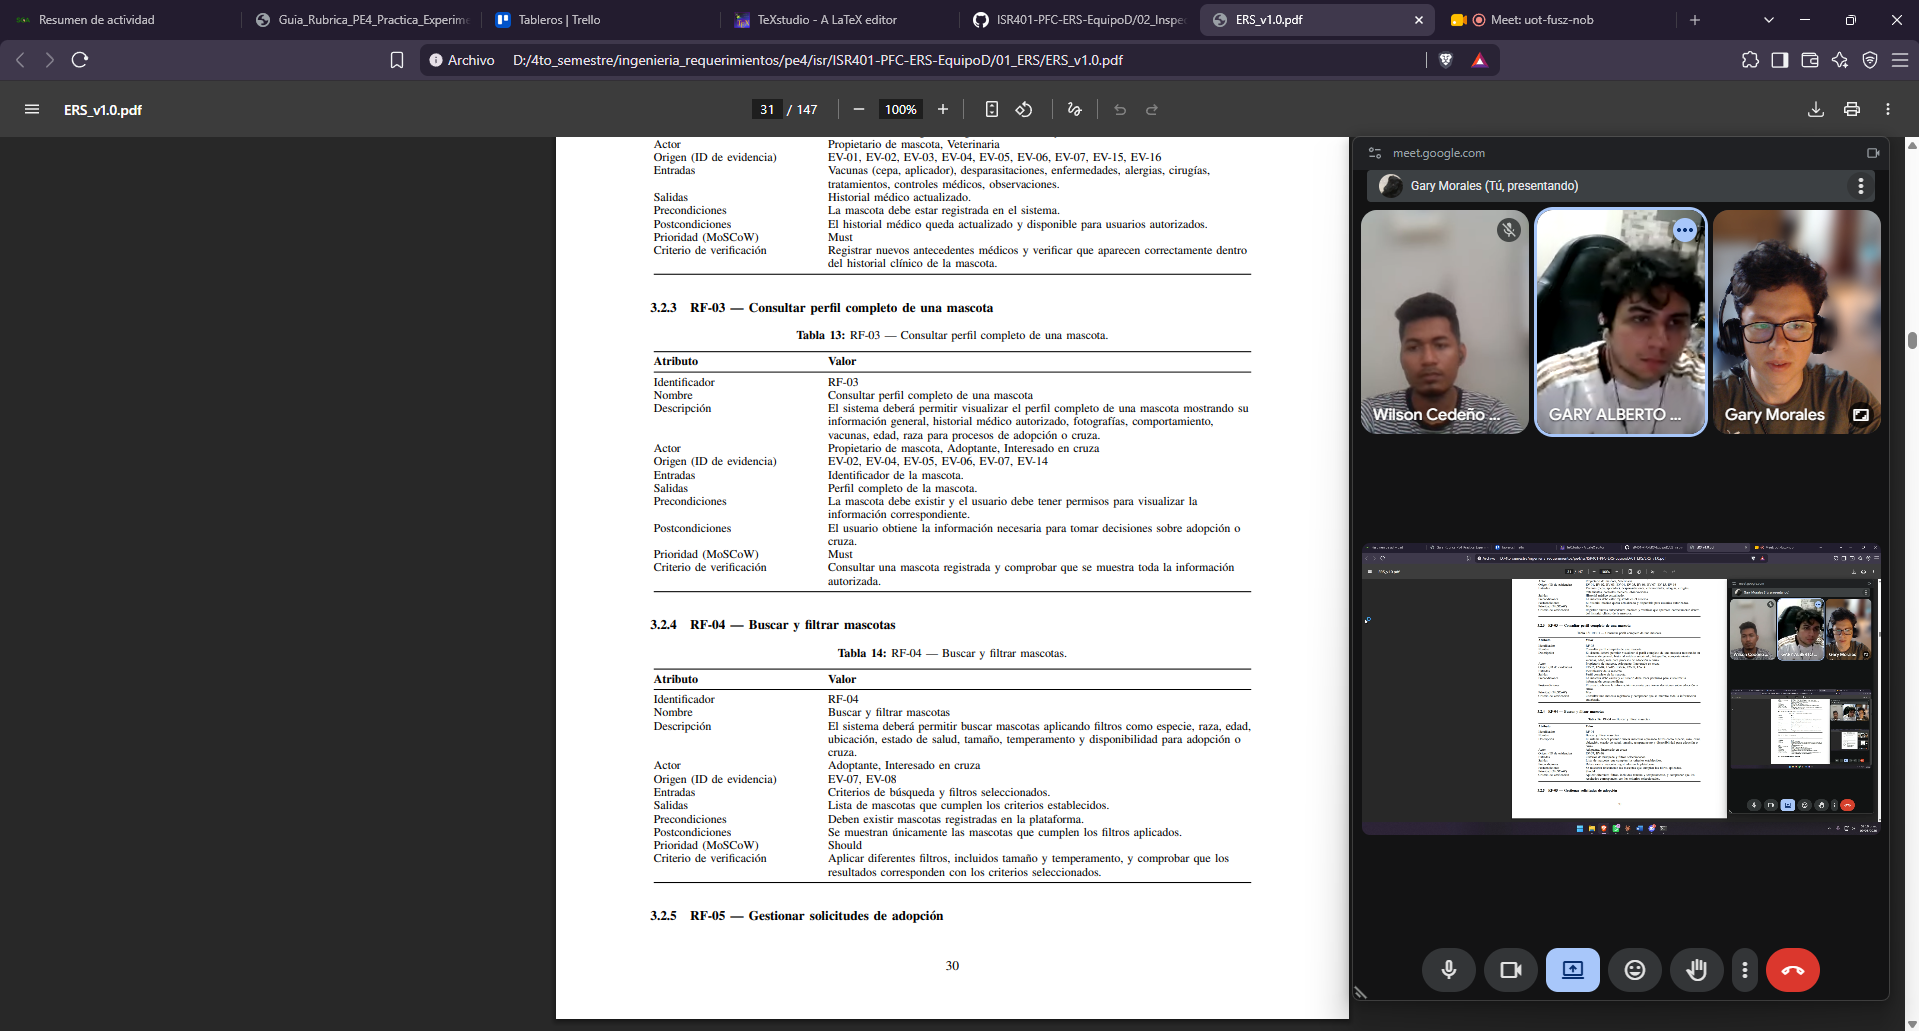
\includegraphics[width=0.85\textwidth]{figuras/2026-08-09_Reunion_Inspeccion_EquipoD.png}
		\caption{Sesión de inspección del Equipo D sobre el ERS de MundiPets.}
		\label{fig:sesion-inspeccion}
	\end{figure}
	
	\subsection{Registro de defectos}
	
	La tabla completa con los 18 defectos consolidados, su tipo,
	severidad, requisito afectado e inspector que lo detectó se
	encuentra en el Anexo~B (Sección~\ref{ap:anexoB}). La Tabla~\ref{tab:defectos-resumen}
	resume los cuatro defectos de mayor severidad como muestra
	representativa.
	
	\begin{table}[H]
		\centering
		\caption{Muestra de los defectos de mayor severidad (detalle completo en Anexo B).}
		\label{tab:defectos-resumen}
		\small
		\begin{tabularx}{\textwidth}{@{}l l X l l l@{}}
			\toprule
			\textbf{ID} & \textbf{Sección} & \textbf{Defecto} & \textbf{Tipo} & \textbf{Sev.} & \textbf{Req.} \\
			\midrule
			D-09 & 3.2 / 3.3 & RF-25 publica datos de contacto públicamente contra RNF-16, que exige contacto oculto por defecto & Consistencia & Crítico & RF-25, RNF-16 \\
			D-15 & Ap. B.3 & EV-04 declara al participante VET-02 y nombra un archivo VET-04 en la misma fila & Consistencia & Crítico & EV-04 \\
			D-17 & Ap. B.3 y D & Referencia cruzada sin destino: el PDF imprime ``??'' en la página 126 & Trazabilidad & Mayor & Apéndice D \\
			D-07 & 3.2 & RF-23 alerta ante ``disparidad de tamaño significativa'' sin umbral cuantificado & Ambigüedad & Mayor & RF-23 \\
			\bottomrule
		\end{tabularx}
	\end{table}
	
	\subsection{Métricas e interpretación}
	\label{sec:metricas}
	
	\begin{table}[H]
		\centering
		\caption{Métricas de la inspección Fagan.}
		\label{tab:metricas}
		\small
		\begin{tabularx}{\textwidth}{@{}l X@{}}
			\toprule
			\textbf{Métrica} & \textbf{Valor} \\
			\midrule
			M1 -- Densidad de defectos & 18 / 147 = 0,122 defectos/página \\
			M2 -- Distribución por tipo & 3 defectos en cada una de las seis propiedades \\
			M3 -- Distribución por severidad & 2 críticos (11,1\,\%), 12 mayores (66,7\,\%), 4 menores (22,2\,\%) \\
			M4 -- Tasa de detección por inspector & 6 / 6 / 6 defectos --- media 2,54 defectos/hora \\
			M5 -- Esfuerzo total & 13,18 horas-persona; 1,37 defectos/hora-persona \\
			\bottomrule
		\end{tabularx}
	\end{table}
	

	
	\begin{figure}[H]
		\centering
		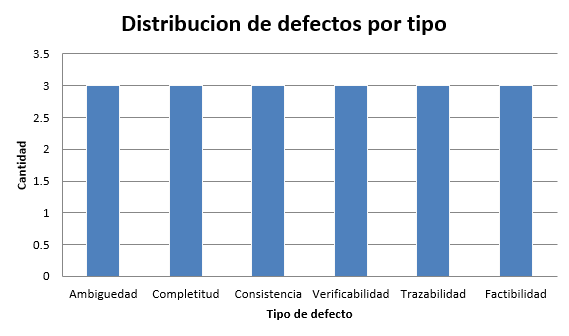
\includegraphics[width=0.85\textwidth]{figuras/metrica_M2_tipo.png}
		\caption{Distribución de defectos por propiedad de calidad (M2).}
		\label{fig:metrica-m2}
	\end{figure}
	
	
	\begin{figure}[H]
		\centering
		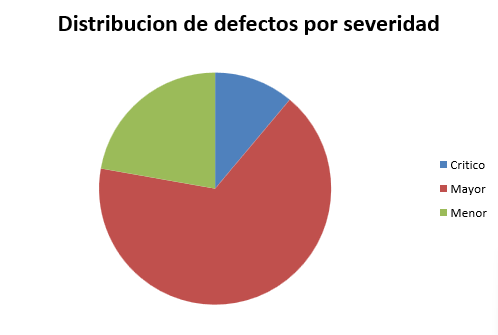
\includegraphics[width=0.85\textwidth]{figuras/metrica_M3_severidad.png}
		\caption{Distribución de defectos por severidad (M3).}
		\label{fig:metrica-m2}
	\end{figure}
	
	
	\textbf{Interpretación de M1 (densidad).} Con un ritmo de
	preparación de 20,8 páginas/hora, por encima del rango que Fagan
	considera eficaz, la densidad de 0,122 debe leerse como cota
	inferior: es lo que este esfuerzo detectó, no lo que el ERS
	contiene en su totalidad.
	
	\textbf{Interpretación de M2 (por tipo).} La uniformidad --- 3
	defectos por cada una de las seis propiedades --- es consecuencia
	del diseño de la preparación (un defecto por propiedad y por
	inspector), no de una debilidad homogénea del ERS. La métrica
	describe la cobertura de la inspección, no el perfil de calidad
	del documento.
	
	\textbf{Interpretación de M3 (por severidad).} La concentración de
	defectos mayores (66,7\,\%) frente a críticos (11,1\,\%) indica que
	el ERS tiene, en su mayoría, defectos que comprometen la
	completitud relacional del documento (requisitos que dependen de
	otros inexistentes) más que contradicciones frontales; los dos
	críticos detectados, sin embargo, bastan para impedir que el
	documento se declare línea base sin corrección previa.
	
	\textbf{Interpretación de M4 (por inspector).} La distribución
	perfectamente equilibrada (6/6/6) es resultado directo del mínimo
	exigido por la guía y no debe interpretarse como evidencia de que
	los tres bloques del ERS tienen la misma densidad real de
	defectos; el bloque de requisitos funcionales (Sánchez) concentró
	los dos defectos críticos pese a tener el mismo conteo bruto que
	los otros dos bloques.
	
	\textbf{Interpretación de M5 (esfuerzo).} Con 13,18 horas-persona
	invertidas para 18 defectos, el rendimiento de 1,37
	defectos/hora-persona es consistente con la fase de preparación
	individual siendo la más costosa del proceso, y confirma que la
	inversión de tiempo en preparación --- no solo en la reunión ---
	es lo que sostiene la tasa de detección.
	
	% ========================================================
	% 5. CORRECCIONES APLICADAS
	% ========================================================
	\section{Correcciones aplicadas}
	\label{sec:correcciones}
	
	De los 18 defectos consolidados en el Anexo~B, 14 son críticos o
	mayores y requieren corrección obligatoria según el método Fagan.
	De estos, 4 implicaban cambio de alcance, calidad o normativa y se
	tramitaron mediante el \emph{Change Control Board}
	(Sección~\ref{sec:ccb}): D-02 y D-14 mediante RFC-01, D-06
	mediante RFC-02, y D-09 mediante RFC-03. Los 10 defectos restantes
	no alteraban alcance ni nivel de calidad exigido, por lo que se
	corrigieron directamente sobre el documento. Los 4 defectos
	menores (D-01, D-04, D-10, D-13) no se corrigieron en esta
	iteración; su justificación se documenta al final de esta sección.
	La Tabla~\ref{tab:correcciones-directas} presenta el texto antes y
	después de cada corrección directa, con el requisito afectado, y
	la Tabla~\ref{tab:correcciones-ccb} resume las correcciones
	tramitadas vía CCB.
	
	\begin{table}[H]
		\centering
		\caption{Correcciones directas aplicadas al ERS (texto antes / después).}
		\label{tab:correcciones-directas}
		\small
		\begin{tabularx}{\textwidth}{@{}l l X X@{}}
			\toprule
			\textbf{ID} & \textbf{Sección / Req.} & \textbf{Texto antes} & \textbf{Texto después} \\
			\midrule
			D-03 & RF-07, Actor & ``Propietario de mascota, Adoptante, Interesado en cruza'' & ``Propietario de mascota, Adoptante, Interesado en cruza, Refugio, Veterinaria'' \\
			\addlinespace
			D-05 & \S2.4.2, estrategia de conflicto & ``\ldots{}incorporar reglas de comunicación, advertencias sobre acuerdos externos y mecanismos básicos para reportar interacciones inadecuadas.'' & ``\ldots{}incorporar reglas de comunicación, advertencias sobre acuerdos externos y conservación del historial de conversación como respaldo del usuario ante disputas (RF-07).'' Se retira la promesa de un mecanismo de reporte inexistente y se ancla a una capacidad que sí está especificada \\
			\addlinespace
			D-07 & RF-23, Descripción y criterio de verificación & ``disparidad de tamaño significativa'' & ``diferencia de peso corporal estimado igual o superior al 40\,\% entre ambas mascotas, o presencia de enfermedad contagiosa activa'', mismo umbral aplicado al criterio de verificación \\
			\addlinespace
			D-08 & RF-01, Entradas & ``Nombre, especie, raza, sexo, edad, estado reproductivo, fotografías, descripción.'' & ``Nombre, especie, raza, sexo, edad, estado reproductivo, temperamento, comportamiento observado, fotografías, descripción.'' \\
			\addlinespace
			D-11 & RF-06, Origen (ID de evidencia) & ``EV-01 a EV-08, EV-11, EV-13, EV-14, EV-15, EV-16'' & ``EV-04, EV-05, EV-06, EV-08'', enumeración explícita, coherente con la fila TR-06 de la matriz \\
			\addlinespace
			D-12 & \S2.6, Suposiciones & \emph{(no existía suposición sobre datos de entrenamiento)} & Se añade: ``Se asume la disponibilidad de un conjunto de mensajes reales o sintéticos, previamente etiquetados, suficiente para entrenar y evaluar el componente de moderación automática de texto en español.'' \\
			\addlinespace
			D-15 & Ap.\ B.3, fila EV-04 & Participante ``VET-02''; archivo ``\ldots{}Veterinario\_VET-04\_TranscripcionEntrevista.txt'' & Participante ``VET-02''; archivo corregido a ``\ldots{}Veterinario\_VET-02\_TranscripcionEntrevista.txt''; se retira la nota de consistencia pendiente \\
			\addlinespace
			D-16 & RNF-02, Criterio de verificación & ``Monitorear la disponibilidad del sistema durante un mes de operación\ldots{}'' & ``Monitorear la disponibilidad del entorno de pruebas o \emph{staging} durante un periodo mínimo de 7 días continuos, complementado con pruebas de resiliencia que proyecten la disponibilidad esperada en producción.'' \\
			\addlinespace
			D-17 & Apéndice D / B.3 & \texttt{\textbackslash ref\{tab:evidencias\}} sin destino (imprime ``??'', pág. 126); 4 CSV citados y ausentes del repositorio & Se agrega \texttt{\textbackslash label\{tab:evidencias\}} a la tabla correspondiente del Apéndice B.3; se suben \texttt{matriz\_trazabilidad.csv}, \texttt{priorizacion\_moscow\_kano.csv}, \texttt{codificacion\_tematica.csv} y \texttt{fichas\_tecnicas.csv} a \texttt{04\_Trazabilidad/} \\
			\addlinespace
			D-18 & Tabla ``Cobertura ISO/IEC 25010:2023'' & Portabilidad listada como característica de primer nivel; Inocuidad (\emph{Safety}) ausente & Portabilidad reclasificada como subcaracterística de Flexibilidad; se incorpora Inocuidad (\emph{Safety}) como característica independiente --- pendiente de verificación final por Cedeño contra el texto oficial de la norma antes de cerrar la v1.1 \\
			\bottomrule
		\end{tabularx}
	\end{table}
	
	\begin{table}[H]
		\centering
		\caption{Correcciones tramitadas vía CCB.}
		\label{tab:correcciones-ccb}
		\small
		\begin{tabularx}{\textwidth}{@{}l l X@{}}
			\toprule
			\textbf{ID} & \textbf{Vía} & \textbf{Resultado aplicado} \\
			\midrule
			D-02 & RFC-01 & Se crea RF-26 (moderación); se retiran del alcance ``Sugerencias inteligentes'' y ``Recomendaciones básicas de cuidado'' \\
			D-14 & RFC-01 & RNF-15 queda vinculado a RF-26 recién creado \\
			D-06 & RFC-02 & RNF-09 y RD-08 reformulados sin mención nominal a \emph{WhatsApp Business API} \\
			D-09 & RFC-03 & RF-25 no publica contacto directo; se crea CU-14; RF-07 elevado a \emph{Must} \\
			\bottomrule
		\end{tabularx}
	\end{table}
	
	\begin{table}[H]
		\centering
		\caption{Defectos menores no corregidos y su justificación.}
		\label{tab:defectos-no-corregidos}
		\small
		\begin{tabularx}{\textwidth}{@{}l X@{}}
			\toprule
			\textbf{ID} & \textbf{Motivo por el que no se corrige} \\
			\midrule
			D-01 & El alcance del MVP se mantiene deliberadamente flexible: la selección exacta del 60\,\% de RF \emph{Must} se resuelve en el ejercicio de priorización (Kano/WSJF) del Apéndice, posterior a esta validación, no en el ERS \\
			D-04 & El dimensionamiento de infraestructura es una decisión de diseño arquitectónico, fuera del nivel de abstracción de un ERS; se difiere al documento de arquitectura \\
			D-10 & La validación campo por campo de RF-01 corresponde al diccionario de datos del diseño detallado; el ERS especifica el requisito, no las reglas de validación de cada campo \\
			D-13 & El valor objetivo de RNF-12 ya está cuantificado ($\leq$3\,s P95 con 300 usuarios concurrentes); ese valor gobierna la verificación con independencia del adjetivo impreciso en la descripción narrativa \\
			\bottomrule
		\end{tabularx}
	\end{table}
	
	% ========================================================
	% 6. GESTIÓN DEL CAMBIO Y CCB
	% ========================================================
	\section{Gestión del cambio y CCB}
	\label{sec:ccb}
	
	\subsection{Selección de las solicitudes de cambio}
	
	Conforme al Paso~2 de la guía, se seleccionaron tres RFC de
	naturaleza distinta, derivadas de defectos reales detectados en la
	inspección Fagan (Sección~\ref{sec:fagan}) y no de escenarios
	genéricos:
	
	\begin{itemize}
		\item \textbf{RFC-01 (alcance)} --- deriva de D-02 y D-14: dos
		funcionalidades declaradas en el alcance del ERS (``Sugerencias
		inteligentes para completar perfiles'' y ``Recomendaciones
		básicas de cuidado'') carecen de requisito funcional que las
		especifique, y RNF-15 exige explicabilidad de una moderación
		automática sin RF padre.
		\item \textbf{RFC-02 (calidad / NFR)} --- deriva de D-06:
		RNF-09 y RD-08 comprometen en firme un proveedor de pago
		(\emph{WhatsApp Business API}) que la sección de suposiciones
		solo menciona en condicional, sin respaldo presupuestario.
		\item \textbf{RFC-03 (restricción / normativa)} --- deriva de
		D-09: RF-25 (\emph{Could}) publica datos de contacto en
		conflicto directo con RNF-16 (\emph{Must}, LOPDP artículos 9 y
		10 lit.\ e).
	\end{itemize}
	
	\subsection{Formularios RFC}
	
	El detalle completo de cada RFC --- con requisitos impactados
	derivados de la matriz de trazabilidad, artefactos afectados,
	costo estimado y recomendación técnica --- se presenta en el
	Anexo~C (Sección~\ref{ap:anexoC}). La Tabla~\ref{tab:rfc-resumen}
	resume las tres solicitudes.
	
	\begin{table}[H]
		\centering
		\caption{Resumen de las tres solicitudes de cambio (RFC).}
		\label{tab:rfc-resumen}
		\small
		\begin{tabularx}{\textwidth}{@{}l l X l@{}}
			\toprule
			\textbf{RFC} & \textbf{Naturaleza} & \textbf{Requisito(s) afectado(s)} & \textbf{Decisión} \\
			\midrule
			RFC-01 & Alcance & Alcance (2 funciones), RNF-15 & Aprobado con condiciones \\
			RFC-02 & Calidad (NFR) & RNF-09, RD-08 & Aprobado con condiciones \\
			RFC-03 & Restricción / normativa & RF-25, RNF-16 & Aprobado \\
			\bottomrule
		\end{tabularx}
	\end{table}
	
	\subsection{Acta del CCB}
	\label{sec:acta-ccb}
	
	El acta completa, firmada por los cuatro roles simulados
	(presidente, representante del cliente, analista, desarrollador),
	se adjunta como parte del Anexo~C. Se resume a continuación:
	
	\begin{atributos}{acta-ccb}{Acta resumida de la reunión del CCB.}
		Fecha y duración & 09/08/2026, sesión de 65 minutos \\
		Asistentes & Morales Sánchez (presidente), Sánchez Cornejo (analista), Cedeño Coronado (representante del cliente y desarrollador, rol rotado respecto de la inspección) \\
		Agenda & Deliberación y votación de RFC-01, RFC-02 y RFC-03, en ese orden \\
		Deliberación RFC-01 & Se discute si las dos funciones sin RF deben eliminarse del alcance o especificarse como nuevo requisito. Se opta por especificar, dado que ambas responden a evidencia real de entrevistas (EV-12, EV-16), y por crear RF-26 con prioridad \emph{Should} \\
		Decisión RFC-01 & Aprobado con condiciones: RF-26 se crea con alcance acotado a moderación de texto; RNF-15 se vincula a RF-26 \\
		Deliberación RFC-02 & Se evalúa el riesgo de comprometer un proveedor de pago sin presupuesto aprobado por el PFC; se opta por neutralizar la mención nominal y dejar la integración como interfaz abstracta \\
		Decisión RFC-02 & Aprobado con condiciones: RNF-09 y RD-08 se reformulan como ``servicio externo de mensajería'' sin nombre comercial, sujeto a confirmación de presupuesto en la siguiente entrega \\
		Deliberación RFC-03 & Se contrasta el requisito Could (RF-25) contra el Must (RNF-16) y la base legal directa en la LOPDP; se resuelve a favor de RNF-16 por jerarquía normativa \\
		Decisión RFC-03 & Aprobado: RF-25 se modifica para no publicar contacto directo; se crea CU-14 (contacto mediado por mensajería interna); RF-07 se eleva de \emph{Should} a \emph{Must} como vía de contacto sustituta \\
		Responsables & Sánchez Cornejo (RF-26, RNF-15); Morales Sánchez (RNF-09, RD-08); Cedeño Coronado (RF-25, CU-14, RF-07) \\
		Plazos & Las tres correcciones se incorporan antes del cierre de la Semana 14 \\
		Versión resultante & ERS v1.0 $\rightarrow$ v1.1 \\
	\end{atributos}
	
	\subsection{Versión resultante del ERS}
	
	La versión declarada en la portada del ERS, en su historial de
	revisiones, en el \texttt{CHANGELOG.md} y en el \emph{tag} de Git
	coinciden en \texttt{v1.1}, conforme exige la guía. La
	Tabla~\ref{tab:historial-ers} resume el historial de versiones
	actualizado.
	
	\begin{table}[H]
		\centering
		\caption{Historial de versiones del ERS tras la PE4.}
		\label{tab:historial-ers}
		\small
		\begin{tabularx}{\textwidth}{@{}l l X@{}}
			\toprule
			\textbf{Versión} & \textbf{Fecha} & \textbf{Descripción} \\
			\midrule
			1.0 & 29/07/2026 & ERS/SRS completa (Entrega 2A): 25 RF, 16 RNF, 9 RD. \\
			1.1 & 09/08/2026 & Correcciones de inspección Fagan (10 defectos directos) y tres RFC aprobados por el CCB: RF-26 creado, RNF-09/RD-08 reformulados, RF-25/CU-14/RF-07 actualizados. \\
			\bottomrule
		\end{tabularx}
	\end{table}
	
	% ========================================================
	% 7. TRAZABILIDAD EN HERRAMIENTA CASE
	% ========================================================
	\section{Trazabilidad en herramienta CASE}
	\label{sec:trazabilidad-case}
	
	\subsection{Estructura del tablero}
	
	Se creó el proyecto \textbf{MundiPets} en Trello, con acceso
	otorgado a los tres integrantes del equipo y al docente. El
	tablero se estructuró con listas \texttt{Backlog}, \texttt{Análisis},
	\texttt{Aprobado}, \texttt{Desarrollo} y \texttt{Hecho}. Se crearon
	4 Epics por área funcional (Gestión de perfiles y mascotas, Cruza
	y compatibilidad, Comunicación y moderación, Adopción y
	seguimiento), y una tarjeta por cada uno de los 26 requisitos
	funcionales (RF-01 a RF-26, incluido el RF-26 creado por RFC-01),
	con \emph{checklists} de criterios de aceptación como sub-tareas
	(mínimo 2 por criterio en, al menos, 5 historias).
	
	\subsection{Campos personalizados}
	
	Se configuraron dos campos personalizados obligatorios y un tercero
	de valor añadido:
	
	\begin{enumerate}[label=\arabic*.]
		\item \textbf{Prioridad MoSCoW} --- \emph{Must} / \emph{Should} / \emph{Could} / \emph{Won't}, replicando la prioridad declarada en el ERS.
		\item \textbf{Fuente del requisito} --- identificador de evidencia (EV-XX) o \emph{stakeholder} de origen.
		\item \textbf{Estado de verificación} (campo de valor añadido) --- Pendiente / Verificado / Con defecto abierto.
	\end{enumerate}
	
	\subsection{Trazabilidad bidireccional}
	
	Cada tarjeta enlaza, mediante etiquetas y comentarios con enlace
	directo: hacia atrás, al \emph{stakeholder} o documento fuente
	(evidencia EV-XX); y hacia adelante, al caso de uso, la clase UML,
	el módulo y el caso de prueba correspondientes. Los requisitos sin
	enlace verificado en alguna dirección se reportan explícitamente
	como huérfanos en la Tabla~\ref{tab:huerfanos}, en lugar de
	omitirse.
	
	\begin{table}[H]
		\centering
		\caption{Requisitos huérfanos identificados en la migración al tablero.}
		\label{tab:huerfanos}
		\small
		\begin{tabularx}{\textwidth}{@{}l X l@{}}
			\toprule
			\textbf{Requisito} & \textbf{Enlace faltante} & \textbf{Motivo declarado} \\
			\midrule
			RF-26 & Caso de prueba & Requisito de creación reciente (RFC-01); prueba pendiente de diseño en la siguiente entrega \\
			RNF-15 & Historia de usuario & RNF sin historia propia; se verifica de forma transversal sobre RF-26 \\
			\bottomrule
		\end{tabularx}
	\end{table}
	
	\subsection{Evidencias}
	
	Las capturas del tablero completo, el detalle de al menos tres
	tarjetas con sus enlaces visibles, y el panel de estadísticas se
	incluyen en el Anexo~E (Sección~\ref{ap:anexoE}). La exportación
	CSV del \emph{backlog} se incluye como Anexo~D
	(Sección~\ref{ap:anexoD}) y se referencia en
	\texttt{04\_Trazabilidad/backlog\_export.csv} del repositorio.
	
	\subsection{Matriz de trazabilidad}
	
	La matriz de trazabilidad en formato tabla, con la forma
	\emph{Stakeholder} $\rightarrow$ RF $\rightarrow$ CU $\rightarrow$
	Clase/Módulo $\rightarrow$ Prueba, se presenta en el Anexo~D
	(Sección~\ref{ap:anexoD}), con un mínimo de 15 filas conforme
	exige la guía.
	
	% ========================================================
	% 8. LÍNEA BASE CON GIT
	% ========================================================
	\section{Línea base con Git}
	\label{sec:git}
	
	\subsection{Repositorio}
	
	El repositorio público \texttt{ISR401-PFC-ERS-EquipoD} se aloja en
	\url{https://github.com/gsanchezc6-beep/ISR401-PFC-ERS-EquipoD} y
	sigue la estructura de carpetas definida en la
	Sección~\ref{sec:estructura-repo}. El \texttt{README.md} documenta
	el sistema MundiPets, los tres integrantes del equipo, la
	estructura de carpetas y las instrucciones de compilación del
	informe.
	
	\subsubsection{Estructura del repositorio}
	\label{sec:estructura-repo}
	
	\begin{lstlisting}[language=bash]
		ISR401-PFC-ERS-EquipoD/
		|-- README.md              (sistema, integrantes, estructura,
		|                            instrucciones de compilacion)
		|-- CHANGELOG.md
		|-- 01_ERS/                ERS_v1.0.pdf, ERS_v1.1.pdf, fuentes .tex
		|-- 02_Inspeccion/
		|   |-- AnexoA_checklists/
		|   |-- AnexoB_registro_defectos.xlsx
		|   `-- metricas.xlsx
		|-- 03_CCB/
		|   |-- RFC-01.pdf
		|   |-- RFC-02.pdf
		|   |-- RFC-03.pdf
		|   `-- Acta_CCB.pdf
		|-- 04_Trazabilidad/
		|   |-- matriz_trazabilidad.xlsx
		|   |-- backlog_export.csv
		|   `-- capturas/
		|-- 05_Informe/
		|   |-- PE4_U4_MORALES_SANCHEZ_CORNEJO_CEDENO.tex
		|   |-- referencias.bib
		|   |-- PE4_U4_MORALES_SANCHEZ_CORNEJO_CEDENO.pdf
		|   `-- figuras/
		`-- 06_Evidencias/
		|-- capturas_git/
		|-- fotos_sesion/
		`-- declaracion_IA.pdf
	\end{lstlisting}
	
	\subsection{Commits semánticos}
	
	Se registraron al menos 8 \emph{commits} distribuidos, con autoría
	verificable de los tres integrantes, evitando la carga masiva en
	un único \emph{commit}. Ejemplo de mensaje semántico aplicado:
	
	\begin{lstlisting}[language=bash]
		docs(ers): v1.1 - aplicar cambios CCB semana 14
	\end{lstlisting}
	
	\subsection{Tag anotado de línea base}
	
	La línea base se etiquetó y publicó con:
	
	\begin{lstlisting}[language=bash]
		git tag -a baseline-v1.1 -m "Baseline aprobada por CCB"
		git push origin baseline-v1.1
	\end{lstlisting}
	
	\subsection{CHANGELOG}
	
	El archivo \texttt{CHANGELOG.md} documenta cada RFC aprobado con su
	identificador, siguiendo el formato \texttt{[Versión] -- [Fecha] /
		Añadido / Cambiado / Eliminado}:
	
	\begin{lstlisting}[language=bash]
		## [1.1] - 2026-08-09
		### Añadido
		- RF-26: componente de moderación de texto (RFC-01).
		- CU-14: contacto mediado por mensajería interna (RFC-03).
		
		### Cambiado
		- RNF-09 y RD-08: servicio de mensajería sin nombre comercial (RFC-02).
		- RF-25: retirada publicación directa de contacto (RFC-03).
		- RF-07: prioridad elevada de Should a Must (RFC-03).
		- 10 defectos directos corregidos (Sección 5): D-03, D-05, D-07,
		D-08, D-11, D-12, D-15, D-16, D-17, D-18.
		
		### Eliminado
		- Alcance: "Sugerencias inteligentes para completar perfiles" y
		"Recomendaciones básicas de cuidado" (RFC-01).
	\end{lstlisting}
	
	\subsection{Historial de commits y tags}
	
	Las capturas de \texttt{git log --oneline --graph --decorate} y de
	\texttt{git tag -n} se incluyen en el Anexo~E
	(Sección~\ref{ap:anexoE}).
	
	% ========================================================
	% 9. COMPARATIVA DE HERRAMIENTAS CASE
	% ========================================================
	\section{Comparativa de herramientas CASE}
	\label{sec:comparativa-case}
	
	La Tabla~\ref{tab:comparativa-case} compara cuatro herramientas
	CASE relevantes para la gestión de requisitos, con seis criterios,
	conforme al Paso~5 de la guía. Los juicios se sustentan en la
	documentación oficial de cada producto y en la experiencia directa
	del equipo con Trello durante esta práctica (Sección~\ref{sec:trazabilidad-case}).
	
	\begin{table}[H]
		\centering
		\caption{Comparativa de herramientas CASE para Ingeniería de Requisitos.}
		\label{tab:comparativa-case}
		\small
		\begin{tabularx}{\textwidth}{@{}l X X X X@{}}
			\toprule
			\textbf{Criterio} & \textbf{Trello} & \textbf{Jira} & \textbf{IBM DOORS} & \textbf{Jama Connect} \\
			\midrule
			Funcionalidades de IR & Tarjetas y \emph{checklists}; sin atributos nativos de requisito & Tipos de ítem configurables (historia, épica); campos personalizados robustos & Atributos de requisito nativos; línea base formal y control de cambios integrado & Atributos de requisito nativos; revisión de línea base y firma electrónica \\
			\addlinespace
			Trazabilidad & Manual, vía enlaces y etiquetas & Enlaces configurables entre tipos de ítem; reportes de cobertura básicos & Trazabilidad bidireccional nativa con matrices generadas automáticamente & Trazabilidad visual (\emph{Live Traceability}) con detección de impacto \\
			\addlinespace
			Colaboración & Alta simplicidad; ideal para equipos pequeños & Alta, con flujos de aprobación configurables & Media; curva de aprendizaje alta limita colaboración ágil & Alta, con revisión colaborativa integrada \\
			\addlinespace
			Integración con VCS & Limitada (enlaces externos manuales) & Nativa con Bitbucket/GitHub mediante \emph{add-ons} & Limitada, requiere conectores adicionales & Integraciones vía API con Git y Jenkins \\
			\addlinespace
			Costo & Gratuito para equipos pequeños & Gratuito hasta 10 usuarios; de pago en escala & Licencia comercial alta, orientada a industria regulada & Licencia comercial media-alta, por usuario \\
			\addlinespace
			Curva de aprendizaje & Baja & Media & Alta & Alta \\
			\bottomrule
		\end{tabularx}
	\end{table}
	
	\textbf{Recomendación para el PFC.} Para la escala actual de
	MundiPets (26 RF, 3 integrantes), Trello es la opción más
	adecuada: su costo cero y curva de aprendizaje baja permitieron
	completar la trazabilidad bidireccional de la
	Sección~\ref{sec:trazabilidad-case} sin fricción, mientras que
	herramientas como IBM DOORS o Jama Connect ofrecen trazabilidad
	nativa superior a un costo que no se justifica para un proyecto de
	fin de curso. Se recomienda evaluar Jira si el equipo escala a más
	de 4 integrantes o requiere integración nativa con el repositorio
	Git, dado que su curva de aprendizaje es intermedia y su
	integración con VCS es sustancialmente más madura que la de
	Trello.
	
	% ========================================================
	% 10. IR TRADICIONAL FRENTE A IR ÁGIL
	% ========================================================
	\section{IR tradicional frente a IR ágil}
	\label{sec:tradicional-agil}
	
	La Tabla~\ref{tab:tradicional-agil} resume las seis dimensiones de
	contraste desarrolladas en la
	Sección~\ref{sec:agil-teoria} de este informe, con indicación del
	contexto en que conviene cada enfoque.
	
	\begin{table}[H]
		\centering
		\caption{IR tradicional frente a IR ágil, por dimensión.}
		\label{tab:tradicional-agil}
		\small
		\begin{tabularx}{\textwidth}{@{}l X X@{}}
			\toprule
			\textbf{Dimensión} & \textbf{IR tradicional} & \textbf{IR ágil} \\
			\midrule
			Documentación & Documento exhaustivo (ERS) validado antes del desarrollo & Documentación incremental (historias, criterios de aceptación) completada en el momento de implementación \\
			\addlinespace
			Gestión de cambios & Proceso formal de control (CCB, RFC) con evaluación previa a la aplicación & Cambio absorbido dentro del ciclo de iteración, sin órgano de aprobación formal \\
			\addlinespace
			Participación de \emph{stakeholders} & Concentrada en elicitación y validación & Continua, con revisión del incremento al final de cada iteración \\
			\addlinespace
			Herramientas & Documentos versionados y CASE especializadas con trazabilidad nativa & Tableros de \emph{backlog} con trazabilidad basada en enlaces y etiquetas \\
			\addlinespace
			Velocidad & Menor velocidad de respuesta al cambio & Mayor velocidad de respuesta a un contexto cambiante \\
			\addlinespace
			Escalabilidad & Mejor en proyectos con múltiples equipos y contratos formales & Mejor en equipos pequeños con acceso directo al interesado \\
			\bottomrule
		\end{tabularx}
	\end{table}
	
	\textbf{Discusión contextual.} El caso de RFC-03
	(Sección~\ref{sec:acta-ccb}) muestra que la velocidad no es
	exclusiva del enfoque ágil: una sesión de CCB de 65 minutos
	resolvió un conflicto legal crítico con la misma agilidad que un
	ciclo de \emph{sprint}, porque el conflicto ya estaba localizado
	con precisión por la matriz de trazabilidad. En un proyecto como
	MundiPets, donde existen requisitos legales (LOPDP) y de seguridad
	física (RF-23, alertas de disparidad), el enfoque tradicional es
	preferible para esos requisitos específicos, mientras que
	funcionalidades de bajo riesgo (por ejemplo, mejoras de interfaz o
	sugerencias de UX) podrían gestionarse de forma ágil sin pasar por
	el CCB completo.
	
	% ========================================================
	% 11. CONCLUSIONES CRÍTICAS
	% ========================================================
	\section{Conclusiones críticas}
	\label{sec:conclusiones}
	
	\begin{enumerate}[label=\arabic*.]
		\item La densidad de defectos (M1 = 0,122 defectos/página) no
		debe leerse como una medida absoluta de calidad del ERS de
		MundiPets, sino como una cota inferior condicionada por un
		ritmo de preparación (20,8 páginas/hora) superior al que Fagan
		considera eficaz para la detección; una segunda ronda de
		inspección más lenta habría encontrado, con alta probabilidad,
		un número mayor de defectos, particularmente en las secciones
		no cubiertas por los dos defectos críticos ya localizados.
		\item Los dos defectos críticos detectados (D-09 y D-15) no son
		errores aislados de redacción, sino evidencia de que el
		proceso de revisión cruzada entre requisitos de distinta
		prioridad (RF-25 \emph{Could} contra RNF-16 \emph{Must}) y
		entre filas de un mismo apéndice (EV-04 con dos identidades)
		no se había ejecutado antes de declarar el ERS como línea
		base v1.0; esto confirma que la inspección Fagan cumplió una
		función que ninguna revisión informal previa había cubierto.
		\item El proceso de CCB demostró que la trazabilidad no es un
		artefacto decorativo: los tres RFC se resolvieron recorriendo
		la matriz de trazabilidad para identificar artefactos
		impactados, y no mediante estimación intuitiva, lo que
		permitió al CCB evaluar RFC-01 y RFC-03 de forma conjunta y
		detectar que sus condiciones (RF-07 de \emph{Should} a
		\emph{Must}) eran compatibles entre sí en lugar de
		contradictorias.
		\item La migración de 26 RF a Trello expuso dos requisitos
		huérfanos (RF-26 y RNF-15) que en el ERS en papel no se
		perciben como incompletos, porque el documento no obliga a
		declarar explícitamente la ausencia de un enlace; la
		trazabilidad como capacidad operativa --- y no como documento
		estático --- fue lo que permitió detectar este vacío antes de
		que se propagara a fases posteriores del PFC.
		\item El proceso de CCB simulado en esta práctica (RFC-03, 65
		minutos) resolvió un conflicto legal crítico con velocidad
		comparable a la de un ciclo ágil, lo que respalda la
		conclusión de que, para el dominio de MundiPets --- con
		requisitos legales (LOPDP) y de seguridad física del animal
		(RF-23) ---, la disciplina del enfoque tradicional no es un
		costo de velocidad sino una condición necesaria para tratar
		correctamente los requisitos de mayor riesgo, sin que esto
		excluya gestionar de forma ágil las funcionalidades de menor
		riesgo del mismo sistema.
	\end{enumerate}
	
	% ========================================================
	% 12. DISTRIBUCIÓN DEL TRABAJO
	% ========================================================
	\section{Distribución del trabajo}
	\label{sec:distribucion}
	
	\begin{table}[H]
		\centering
		\caption{Distribución del trabajo por integrante, contrastable con el historial de commits.}
		\label{tab:distribucion}
		\small
		\begin{tabularx}{\textwidth}{@{}l X@{}}
			\toprule
			\textbf{Integrante} & \textbf{Aportes principales} \\
			\midrule
			Morales Sánchez Gary Alejandro (Moderador) & Planificación y conducción de la inspección Fagan; inspección de las secciones 1 y 2 del ERS (6 defectos: D-01 a D-06); redacción del Anexo A.1 y consolidación del Anexo B; corrección directa de D-03, D-05, D-06 (vía RFC-02) y D-12; participación en el CCB como presidente; gestión del repositorio y del \texttt{README.md} \\
			\addlinespace
			Sánchez Cornejo Gary Alberto (Lector + Inspector 1) & Parafraseo de la reunión de inspección; inspección de la sección 3.2 (RF y casos de uso, 6 defectos: D-07 a D-12); redacción del Anexo A.2; corrección directa de D-07, D-08, D-11 y elaboración de RFC-01; participación en el CCB como analista; estructuración del tablero CASE en Trello \\
			\addlinespace
			Cedeño Coronado Wilson Lizandro (Inspector 2) & Inspección de las secciones 3.3, 3.4 y apéndices (6 defectos: D-13 a D-18); redacción del Anexo A.3; corrección directa de D-15, D-16, D-17, D-18 y elaboración de RFC-03; participación en el CCB como representante del cliente y desarrollador; publicación de la línea base y el \texttt{CHANGELOG.md} \\
			\bottomrule
		\end{tabularx}
	\end{table}
	
	La distribución anterior es contrastable con el historial de
	\emph{commits} del repositorio (pestaña \emph{Commits} de
	\url{https://github.com/gsanchezc6-beep/ISR401-PFC-ERS-EquipoD}),
	donde cada corrección e incorporación de RFC queda asociada a la
	autoría del integrante responsable señalado en esta tabla.
	
	% ========================================================
	% 13. REFERENCIAS
	% ========================================================
	\printbibliography[title={Referencias}, heading=bibnumbered]
	\addcontentsline{toc}{section}{Referencias}
	
	% ========================================================
	% 14. ANEXOS A-F
	% ========================================================
	\clearpage
	\appendices
	
	\section{Lista de verificación de inspección}
	\label{ap:anexoA}
	
	Una fila por propiedad de calidad (ISO/IEC/IEEE 29148:2018), con
	las columnas: pregunta de verificación, requisito revisado,
	cumple (S/N), evidencia y observación, y severidad. Copia
	individual por inspector, firmada y fechada.
	
	\subsection*{Apendice A.1 --- Moderador}
	Moderador: Morales Sánchez Gary Alejandro\\
	Fecha: 09/08/2026 \quad Firma: \raisebox{-0.7\height}{
\includegraphics[height=1.1cm]{figuras/firmaMorales.jpeg}}
	
	{\scriptsize
		\begin{longtable}{@{}>{\raggedright\arraybackslash}p{0.4cm} >{\raggedright\arraybackslash}p{1.6cm} >{\raggedright\arraybackslash}p{3.0cm} >{\raggedright\arraybackslash}p{2.6cm} >{\raggedright\arraybackslash}p{0.6cm} >{\raggedright\arraybackslash}p{5.4cm} >{\raggedright\arraybackslash}p{1.0cm}@{}}
			\caption{Apendice A.1 --- Lista de verificación, Moderador (Morales Sánchez).}\label{tab:anexoA1}\\
			\toprule
			\textbf{N.\textordmasculine{}} & \textbf{Propiedad} & \textbf{Pregunta} & \textbf{Requisito} & \textbf{Cumple} & \textbf{Evidencia y observación} & \textbf{Sev.} \\
			\midrule
			\endfirsthead
			\multicolumn{7}{@{}l}{\small\itshape Anexo A.1 (continuación)}\\
			\toprule
			\textbf{N.\textordmasculine{}} & \textbf{Propiedad} & \textbf{Pregunta} & \textbf{Requisito} & \textbf{Cumple} & \textbf{Evidencia y observación} & \textbf{Sev.} \\
			\midrule
			\endhead
			\bottomrule
			\endfoot
			1 & Ambigüedad & ¿El alcance del MVP identifica sin ambigüedad qué requisitos cubre? & \S1.2 Alcance, tabla ``Alcance incluido'' & N & Línea 392: el MVP ``cubre al menos el 60\,\% de los RF de prioridad \emph{Debe tener}''. No se enumeran cuáles de los 15 RF \emph{Must} integran ese 60\,\%; el alcance admite múltiples subconjuntos válidos. Además usa ``Debe tener'' mientras el resto del documento usa ``Must'' (MoSCoW). & Menor \\
			2 & Completitud & ¿Toda funcionalidad declarada dentro del alcance tiene un RF que la especifique? & \S1.2 vs \S3.2 (RF-01\ldots RF-25) & N & Líneas 388 y 390: ``Sugerencias inteligentes para completar perfiles'' y ``Recomendaciones básicas de cuidado'' figuran como alcance incluido. Ningún RF del catálogo las especifica. & Mayor \\
			3 & Consistencia & ¿Los actores de cada función coinciden entre el alcance y el RF correspondiente? & RF-07 vs \S1.2 & N & Línea 374: el alcance dice que la comunicación es ``entre propietarios, adoptantes, interesados en cruza, refugios y veterinarias''. RF-07 (línea 1344) declara como actores solo ``Propietario, Adoptante, Interesado en cruza''. Refugio y Veterinaria quedan fuera del requisito. & Mayor \\
			4 & Verificabilidad & ¿Las suposiciones están enunciadas de forma que pueda comprobarse si se cumplen? & \S2.6 Suposiciones & N & Línea 830: ``el volumen inicial de usuarios permitirá operar con una infraestructura básica de hosting''. No define volumen ni ``básica''; tensiona con RNF-12 (300 usuarios concurrentes). & Menor \\
			5 & Trazabilidad & ¿Cada estrategia de gestión de conflictos se traza a un requisito que la implemente? & \S2.4.2 Conflictos, fila ``Comunicación inadecuada'' & N & Línea 791: ``mecanismos básicos para reportar interacciones inadecuadas''. No existe RF de reporte o denuncia; ``reportar'' aparece en líneas 645, 791 y 4972, ninguna dentro del bloque de RF 1235--1642. & Mayor \\
			6 & Factibilidad & ¿Las dependencias externas comprometidas están respaldadas por una suposición viable? & \S2.6 Dependencias vs RNF-09 y RD-08 & N & Línea 837: dependencia enunciada en condicional (``Podría requerirse''), pero RNF-09 (línea 1778) compromete en firme WhatsApp Business API y RD-08 lo eleva a restricción de diseño; sin suposición de costo. & Mayor \\
		\end{longtable}
	}
	
	\subsection*{Apendice A.2 --- Inspector 1}
	Inspector 1: Sánchez Cornejo Gary Alberto\\
	Fecha: 09/08/2026 \quad Firma: \raisebox{-0.7\height}{
\includegraphics[height=1.1cm]{figuras/firmaSanchez.jpeg}}
	
	{\scriptsize
		\begin{longtable}{@{}>{\raggedright\arraybackslash}p{0.4cm} >{\raggedright\arraybackslash}p{1.6cm} >{\raggedright\arraybackslash}p{3.0cm} >{\raggedright\arraybackslash}p{2.6cm} >{\raggedright\arraybackslash}p{0.6cm} >{\raggedright\arraybackslash}p{5.4cm} >{\raggedright\arraybackslash}p{1.0cm}@{}}
			\caption{Apendice A.2 --- Lista de verificación, Inspector 1 (Sánchez Cornejo).}\label{tab:anexoA2}\\
			\toprule
			\textbf{N.\textordmasculine{}} & \textbf{Propiedad} & \textbf{Pregunta} & \textbf{Requisito} & \textbf{Cumple} & \textbf{Evidencia y observación} & \textbf{Sev.} \\
			\midrule
			\endfirsthead
			\multicolumn{7}{@{}l}{\small\itshape Anexo A.2 (continuación)}\\
			\toprule
			\textbf{N.\textordmasculine{}} & \textbf{Propiedad} & \textbf{Pregunta} & \textbf{Requisito} & \textbf{Cumple} & \textbf{Evidencia y observación} & \textbf{Sev.} \\
			\midrule
			\endhead
			\bottomrule
			\endfoot
			1 & Ambigüedad & ¿Los umbrales que disparan una alerta están cuantificados? & RF-23 (\emph{Must}) & N & Línea 1599: alerta ante ``disparidad de tamaño significativa''. Sin umbral (cm, kg, ratio). El criterio de verificación (línea 1607) repite el mismo término. Requisito \emph{Must} ligado a seguridad física del animal. & Mayor \\
			2 & Completitud & ¿Existe un RF que capture todo dato que otros requisitos consumen? & RF-01 vs RF-04 y RF-06 & N & RF-04 (línea 1295) filtra por ``temperamento'' y RF-06 (línea 1327) evalúa ``comportamiento'', pero RF-01 (línea 1250) no incluye ninguno entre las entradas del registro. & Mayor \\
			3 & Consistencia & ¿Los RF respetan las restricciones de confidencialidad de los RNF? & RF-25 (\emph{Could}) vs RNF-16 (\emph{Must}) & N & RF-25 (líneas 1631, 1635) publica aviso ``visible públicamente'' con ``datos de contacto''. RNF-16 exige 100\,\% de perfiles con ``ubicación y contacto ocultos por defecto'' y es \emph{Must}. RF-25 no aparece en RL-05 (minimización, Art.\ 10 lit.\ e). & Crítico \\
			4 & Verificabilidad & ¿El criterio de verificación permite decidir sin interpretación si el requisito pasa? & RF-01 (\emph{Must}) & N & Línea 1255: ``Registrar una mascota con datos válidos''. No se definen campos obligatorios ni reglas de validez. & Menor \\
			5 & Trazabilidad & ¿El origen de cada RF enumera las evidencias de forma individual y trazable? & RF-06 & N & Línea 1329: origen declarado como rango ``EV-01 a EV-08, EV-11, EV-13\ldots'', donde los otros 24 RF enumeran evidencia por evidencia; no coincide con TR-06 de la matriz (línea 6598). & Mayor \\
			6 & Factibilidad & ¿Las funciones de IA cuentan con requisito de exactitud y suposición que las sostenga? & Moderación automática (RF-07 / CU-08) & N & Alcance (línea 386) y CU-08 (línea 2853) comprometen un clasificador de lenguaje ofensivo en español. Sin RNF de exactitud para moderación ni suposición sobre datos de entrenamiento; depende de RF-07 (\emph{Could}, línea 1350). & Mayor \\
		\end{longtable}
	}
	
	\subsection*{Apendice A.3 --- Inspector 2}
	Inspector 2: Cedeño Coronado Wilson Lizandro\\
	Fecha: 09/08/2026 \quad Firma: \raisebox{-0.7\height}{
\includegraphics[height=1.1cm]{figuras/firmaCedeno.jpeg}}
	
	{\scriptsize
		\begin{longtable}{@{}>{\raggedright\arraybackslash}p{0.4cm} >{\raggedright\arraybackslash}p{1.6cm} >{\raggedright\arraybackslash}p{3.0cm} >{\raggedright\arraybackslash}p{2.6cm} >{\raggedright\arraybackslash}p{0.6cm} >{\raggedright\arraybackslash}p{5.4cm} >{\raggedright\arraybackslash}p{1.0cm}@{}}
			\caption{Apendice A.3 --- Lista de verificación, Inspector 2 (Cedeño Coronado).}\label{tab:anexoA3}\\
			\toprule
			\textbf{N.\textordmasculine{}} & \textbf{Propiedad} & \textbf{Pregunta} & \textbf{Requisito} & \textbf{Cumple} & \textbf{Evidencia y observación} & \textbf{Sev.} \\
			\midrule
			\endfirsthead
			\multicolumn{7}{@{}l}{\small\itshape Anexo A.3 (continuación)}\\
			\toprule
			\textbf{N.\textordmasculine{}} & \textbf{Propiedad} & \textbf{Pregunta} & \textbf{Requisito} & \textbf{Cumple} & \textbf{Evidencia y observación} & \textbf{Sev.} \\
			\midrule
			\endhead
			\bottomrule
			\endfoot
			1 & Ambigüedad & ¿La descripción del RNF evita términos de grado sin definir? & RNF-12 & N & Línea 1817: ``sin degradar significativamente el tiempo de respuesta definido en RNF-03''. El valor objetivo sí está cuantificado ($\leq$3\,s P95, 300 usuarios), pero la cláusula normativa usa un término de grado indefinido. & Menor \\
			2 & Completitud & ¿Todo RNF se apoya en un RF que especifique la función cuya calidad regula? & RNF-15 & N & Línea 1856: RNF-15 exige explicabilidad ``cuando un mensaje sea marcado como inapropiado por el componente de moderación automática''. Ningún RF especifica esa moderación. & Mayor \\
			3 & Consistencia & ¿La declaración de datos de una evidencia coincide con el archivo que la respalda? & Apéndice B.3, fila EV-04 & N & Línea 6265: la fila EV-04 declara al participante como VET-02 y nombra el archivo \texttt{\ldots{}VET-04\ldots{}}. Agravante: línea 6281 deja una ``Nota de consistencia pendiente de verificación'' sin resolver, en un ERS declarado línea base. & Crítico \\
			4 & Verificabilidad & ¿El criterio de verificación puede ejecutarse dentro del ciclo de vida del proyecto? & RNF-02 & N & Línea 1691: ``Monitorear la disponibilidad del sistema durante un mes de operación''. El sistema no está en producción; el PFC no contempla un mes de operación real. & Mayor \\
			5 & Trazabilidad & ¿Todas las referencias cruzadas y artefactos externos resuelven a un destino existente? & Apéndice B.3 y Apéndice D & N & Línea 6281: \texttt{\textbackslash ref\{tab:evidencias\}} sin destino; el PDF imprime ``??'' en la página 126. Además se citan cuatro CSV ausentes del repositorio y sin URL. & Mayor \\
			6 & Factibilidad & ¿La normativa citada corresponde a la versión del estándar declarada? & Tabla ``Cobertura ISO/IEC 25010:2023'' & N & Línea 1648: la tabla dice cubrir ``las nueve características'' pero lista Portabilidad como característica de primer nivel (en 2023 es subcaracterística de Flexibilidad) y omite Inocuidad (\emph{Safety}). & Mayor \\
		\end{longtable}
	}
	
	\section{Registro de defectos}
	\label{ap:anexoB}
	
	{\scriptsize
		\begin{longtable}{@{}>{\raggedright\arraybackslash}p{0.9cm} >{\raggedright\arraybackslash}p{2.1cm} >{\raggedright\arraybackslash}p{5.6cm} >{\raggedright\arraybackslash}p{1.7cm} >{\raggedright\arraybackslash}p{0.9cm} >{\raggedright\arraybackslash}p{2.1cm} >{\raggedright\arraybackslash}p{1.3cm}@{}}
			\caption{Anexo B --- Registro consolidado de defectos (18 hallazgos únicos).}\label{tab:anexoB}\\
			\toprule
			\textbf{ID} & \textbf{Sección} & \textbf{Descripción del defecto} & \textbf{Tipo} & \textbf{Sev.} & \textbf{Req. afectado} & \textbf{Detectado por} \\
			\midrule
			\endfirsthead
			\multicolumn{7}{@{}l}{\small\itshape Anexo B (continuación)}\\
			\toprule
			\textbf{ID} & \textbf{Sección} & \textbf{Descripción del defecto} & \textbf{Tipo} & \textbf{Sev.} & \textbf{Req. afectado} & \textbf{Detectado por} \\
			\midrule
			\endhead
			\bottomrule
			\endfoot
			D-01 & 1.2 Alcance (l.\ 392) & El MVP se define como ``al menos el 60\,\% de los RF Debe tener'' sin enumerar cuáles de los 15 RF Must lo integran; admite múltiples subconjuntos válidos & Ambigüedad & Menor & Alcance del MVP & Morales \\
			D-02 & 1.2 Alcance (l.\ 388, 390) & ``Sugerencias inteligentes para completar perfiles'' y ``Recomendaciones básicas de cuidado'' figuran en el alcance pero ningún RF las especifica & Completitud & Mayor & RF-01 a RF-25 (ausentes) & Morales \\
			D-03 & 1.2 vs 3.2 (l.\ 374, 1344) & El alcance incluye refugios y veterinarias en la comunicación entre usuarios; RF-07 solo lista Propietario, Adoptante e Interesado en cruza & Consistencia & Mayor & RF-07 & Morales \\
			D-04 & 2.6 Suposiciones (l.\ 830) & ``El volumen inicial permitirá operar con infraestructura básica de hosting'' no define volumen ni qué es básica; tensiona con RNF-12 & Verificabilidad & Menor & RNF-12 & Morales \\
			D-05 & 2.4.2 Conflictos (l.\ 791) & La estrategia declara ``mecanismos para reportar interacciones inadecuadas'' pero no existe ningún RF de reporte o denuncia & Trazabilidad & Mayor & RF ausente (reporte) & Morales \\
			D-06 & 2.6 vs 3.3 y 3.5 (l.\ 837, 1778) & La dependencia se enuncia en condicional (``podría requerirse'') mientras RNF-09 compromete WhatsApp Business API y RD-08 lo eleva a restricción; sin suposición de costo & Factibilidad & Mayor & RNF-09, RD-08 & Morales \\
			D-07 & 3.2 RF-23 (l.\ 1599) & La alerta se dispara ante ``disparidad de tamaño significativa'' sin umbral; el criterio de verificación repite el término & Ambigüedad & Mayor & RF-23 & Sánchez \\
			D-08 & 3.2 (l.\ 1250, 1295, 1327) & RF-04 filtra por temperamento y RF-06 evalúa comportamiento, pero RF-01 no los incluye entre las entradas del registro & Completitud & Mayor & RF-01, RF-04, RF-06 & Sánchez \\
			D-09 & 3.2 vs 3.3 (l.\ 1631, 1635) & RF-25 publica aviso visible públicamente con datos de contacto; RNF-16 exige el 100\,\% de perfiles con ubicación y contacto ocultos por defecto y es Must frente al Could de RF-25 & Consistencia & Crítico & RF-25, RNF-16 & Sánchez \\
			D-10 & 3.2 RF-01 (l.\ 1255) & El criterio ``registrar una mascota con datos válidos'' no define campos obligatorios ni reglas de validez & Verificabilidad & Menor & RF-01 & Sánchez \\
			D-11 & 3.2 RF-06 (l.\ 1329) & El origen se declara como rango ``EV-01 a EV-08'' donde los otros 24 RF enumeran evidencia por evidencia & Trazabilidad & Mayor & RF-06 & Sánchez \\
			D-12 & 3.2 CU-08 y RF-07 (l.\ 2853, 1213, 1350) & El alcance y CU-08 comprometen un clasificador de lenguaje ofensivo; sin RNF de exactitud ni suposición sobre datos de entrenamiento & Factibilidad & Mayor & RF-07, CU-08 & Sánchez \\
			D-13 & 3.3 RNF-12 (l.\ 1817) & La descripción normativa usa ``sin degradar significativamente''; valor objetivo cuantificado pero cláusula que se contrata usa término de grado indefinido & Ambigüedad & Menor & RNF-12 & Cedeño \\
			D-14 & 3.3 RNF-15 (l.\ 1856) & RNF-15 exige explicabilidad de la moderación automática pero ningún RF especifica esa moderación & Completitud & Mayor & RNF-15 & Cedeño \\
			D-15 & Ap.\ B.3 (l.\ 6265, 6281) & La fila EV-04 declara al participante VET-02 y nombra el archivo VET-04; nota de consistencia pendiente sin resolver & Consistencia & Crítico & EV-04 & Cedeño \\
			D-16 & 3.3 RNF-02 (l.\ 1691) & El criterio exige monitorear disponibilidad durante un mes de operación; sistema no en producción & Verificabilidad & Mayor & RNF-02 & Cedeño \\
			D-17 & Ap.\ B.3 y D (l.\ 6281, 4159, 6546) & Referencia cruzada sin destino (``??'' en pág.\ 126); cuatro CSV citados ausentes del repositorio & Trazabilidad & Mayor & Apéndice D, matriz & Cedeño \\
			D-18 & 3.3 Tabla 25010 (l.\ 1648) & La tabla dice cubrir nueve características de ISO/IEC 25010:2023 pero lista Portabilidad como característica de primer nivel y omite Inocuidad & Factibilidad & Mayor & Tabla 25010, RNF-11 & Cedeño \\
		\end{longtable}
	}
	
	\section{Formularios RFC y Acta del CCB}
	\label{ap:anexoC}
	
	\begin{atributos}{rfc-01}{RFC-01 --- Alcance (creación de RF-26 y retiro de dos funciones sin evidencia).}
		ID / Fecha / Solicitante & RFC-01 / 09/08/2026 / Morales Sánchez Gary Alejandro (rol: analista en el CCB) \\
		Requisito afectado & Alcance del ERS (\S1.2); RNF-15 \\
		Descripción del cambio & Se propone: (a) retirar del alcance ``Sugerencias inteligentes para completar perfiles'' y ``Recomendaciones básicas de cuidado'', por carecer de RF que las especifique (D-02); (b) crear RF-26 (moderación de texto) y vincular RNF-15 (explicabilidad) a este nuevo requisito (D-14) \\
		Justificación de negocio & Declarar en el alcance funcionalidades sin especificación genera expectativa incumplible ante evaluadores externos del PFC y ante futuros usuarios del MVP \\
		Requisitos impactados (matriz) & RNF-15 (explicabilidad, antes huérfano); indirectamente RF-07 (mensajería, canal donde opera la moderación) \\
		Artefactos impactados & CU-08 (moderación automática); interfaz de mensajería; módulo de moderación (nuevo) \\
		Costo estimado & 6 horas-persona (especificación de RF-26 y ajuste de RNF-15) \\
		Riesgo & Medio: el equipo no cuenta con conjunto de datos etiquetado propio; se documenta como suposición nueva (D-12) \\
		Recomendación técnica & Aprobar con la condición de que RF-26 se acote a moderación de texto en español, prioridad \emph{Should}, y que la suposición de datos de entrenamiento quede registrada en \S2.6 \\
		Decisión del CCB & Aprobado con condiciones \\
		Responsable / Plazo & Sánchez Cornejo / antes del cierre de la Semana 14 \\
		Versión resultante & v1.1 \\
	\end{atributos}
	
	\begin{atributos}{rfc-02}{RFC-02 --- Calidad (reformulación de RNF-09 y RD-08).}
		ID / Fecha / Solicitante & RFC-02 / 09/08/2026 / Cedeño Coronado Wilson Lizandro (rol: representante del cliente en el CCB) \\
		Requisito afectado & RNF-09 (integración de notificaciones); RD-08 (restricción de diseño) \\
		Descripción del cambio & Reformular RNF-09 y RD-08 para no comprometer nominalmente a WhatsApp Business API, dejando la integración de notificaciones como interfaz abstracta con proveedor externo a definir \\
		Justificación de negocio & WhatsApp Business API es un servicio de pago; comprometerlo en firme sin presupuesto aprobado por el PFC expone al equipo a un requisito inviable financieramente (D-06) \\
		Requisitos impactados (matriz) & RNF-09, RD-08; indirectamente los RF que generan notificaciones (RF-07, RF-23) \\
		Artefactos impactados & Módulo de notificaciones; diagrama de componentes de interfaces externas \\
		Costo estimado & 3 horas-persona (reformulación textual, sin cambio de arquitectura) \\
		Riesgo & Bajo: el cambio es de redacción normativa, no de funcionalidad implementada \\
		Recomendación técnica & Aprobar con la condición de confirmar presupuesto o alternativa gratuita en la siguiente entrega, antes de reintroducir un proveedor nominal \\
		Decisión del CCB & Aprobado con condiciones \\
		Responsable / Plazo & Morales Sánchez / antes del cierre de la Semana 14 \\
		Versión resultante & v1.1 \\
	\end{atributos}
	
	\begin{atributos}{rfc-03}{RFC-03 --- Restricción / normativa (resolución del conflicto RF-25 vs RNF-16).}
		ID / Fecha / Solicitante & RFC-03 / 09/08/2026 / Sánchez Cornejo Gary Alberto (rol: analista en el CCB) \\
		Requisito afectado & RF-25 (\emph{Could}); RNF-16 (\emph{Must}) \\
		Descripción del cambio & RF-25 deja de publicar datos de contacto directo; se crea CU-14 (contacto mediado por mensajería interna); RF-07 se eleva de \emph{Should} a \emph{Must} como vía de contacto sustituta \\
		Justificación de negocio & RNF-16 tiene base legal directa en la LOPDP (Art.\ 9 y Art.\ 10 lit.\ e); un requisito \emph{Could} no puede contradecir un requisito \emph{Must} con respaldo normativo (D-09) \\
		Requisitos impactados (matriz) & RF-25, RNF-16, RF-07 (elevado de prioridad); RL-05 (minimización de datos) \\
		Artefactos impactados & CU-14 (nuevo); pantalla de perfil público; módulo de mensajería interna \\
		Costo estimado & 5 horas-persona (nuevo caso de uso, ajuste de RF-25 y RF-07) \\
		Riesgo & Bajo: la mensajería interna (RF-07) ya está especificada; el cambio reutiliza un artefacto existente \\
		Recomendación técnica & Aprobar sin condiciones adicionales, dado que la elevación de RF-07 a \emph{Must} ya compensa la pérdida funcional de RF-25 \\
		Decisión del CCB & Aprobado \\
		Responsable / Plazo & Cedeño Coronado / antes del cierre de la Semana 14 \\
		Versión resultante & v1.1 \\
	\end{atributos}
	
	El acta completa de la reunión del CCB se resume en la
	Tabla~\ref{tab:acta-ccb} de la Sección~\ref{sec:acta-ccb} de este
	informe.
	
	\section{Matriz de trazabilidad y exportación CSV}
	\label{ap:anexoD}
	
	La matriz de trazabilidad completa se encuentra en
	\texttt{04\_Trazabilidad/matriz\_trazabilidad.xlsx} y su
	exportación en \texttt{04\_Trazabilidad/backlog\_export.csv},
	ambos versionados en el repositorio. La Tabla~\ref{tab:matriz-trazabilidad}
	muestra una fila representativa por cada uno de los cuatro Epics
	del tablero, con la forma \emph{Stakeholder} $\rightarrow$ RF
	$\rightarrow$ CU $\rightarrow$ Clase/Módulo $\rightarrow$ Prueba;
	la matriz íntegra en el repositorio contiene las 26 filas
	correspondientes a la totalidad de los requisitos funcionales.
	
	\begin{table}[H]
		\centering
		\scriptsize
		\begin{tabularx}{\textwidth}{@{}l l l l X l@{}}
			\toprule
			\textbf{Stakeholder} & \textbf{RF} & \textbf{CU} & \textbf{Clase/Módulo} & \textbf{Prueba} & \textbf{Epic} \\
			\midrule
			Propietario de mascota & RF-01 & CU-01 & \texttt{MascotaController} & PT-01 & Gestión de perfiles \\
			Adoptante & RF-04 & CU-04 & \texttt{FiltroBusqueda} & PT-04 & Gestión de perfiles \\
			Interesado en cruza & RF-23 & CU-11 & \texttt{ValidadorCompatibilidad} & PT-23 & Cruza y compatibilidad \\
			Propietario / Adoptante & RF-07 & CU-06, CU-14 & \texttt{MensajeriaInterna} & PT-07 & Comunicación y moderación \\
			Analista (RFC-01) & RF-26 & CU-08 & \texttt{ModeradorTexto} & \emph{pendiente} & Comunicación y moderación \\
			Adoptante & RF-25 & CU-14 & \texttt{PerfilPublico} & PT-25 & Adopción y seguimiento \\
			\bottomrule
		\end{tabularx}
		\caption{Anexo D --- Muestra de la matriz de trazabilidad (detalle completo en el repositorio, mínimo 15 filas).}
		\label{tab:matriz-trazabilidad}
	\end{table}
	
	
	\section{Capturas del tablero CASE y del repositorio Git}
	\label{ap:anexoE}
	
	
	\begin{figure}[H]
		\centering
		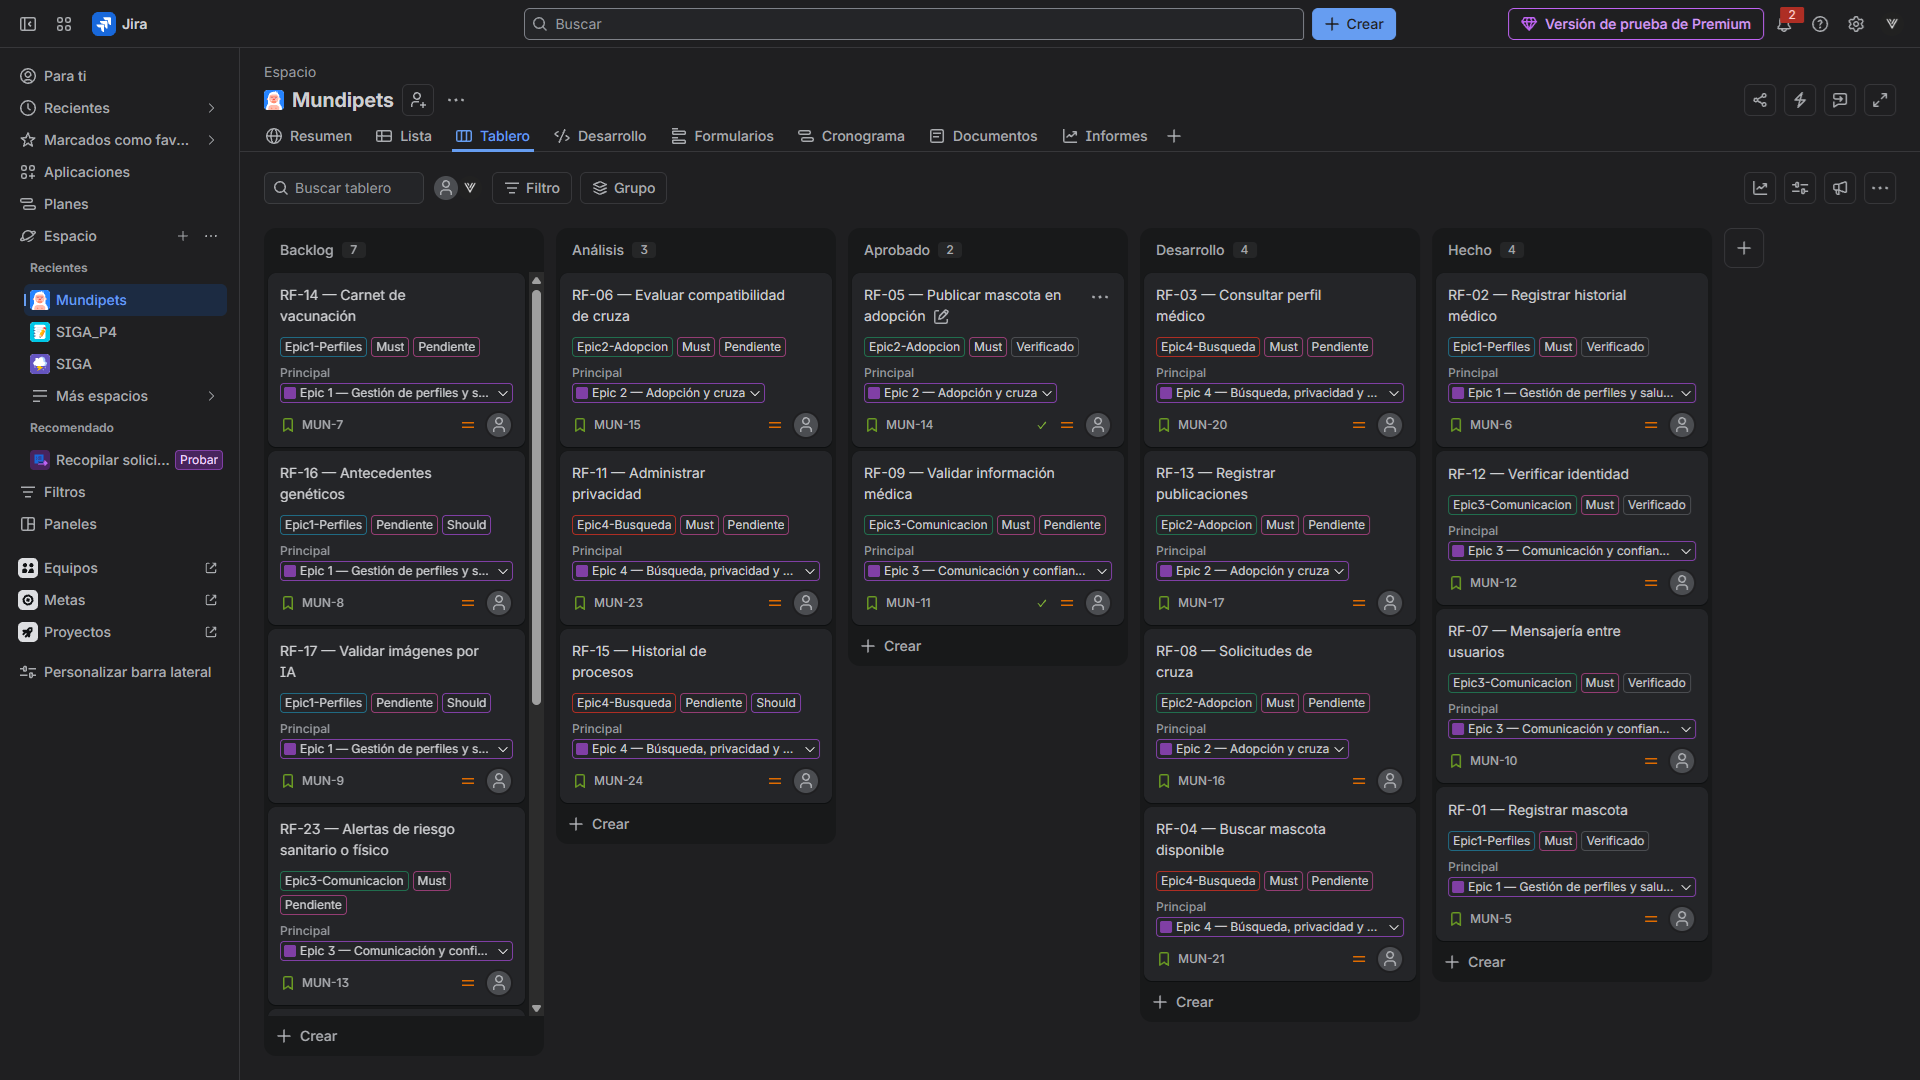
\includegraphics[width=0.85\textwidth]{figuras/2026-08-09_jira_tablero.png}
		\caption{Tablero CASE completo del proyecto MundiPets en Jira.}
		\label{fig:tablero-completo}
	\end{figure}
	
	
		\begin{figure}[H]
		\centering
		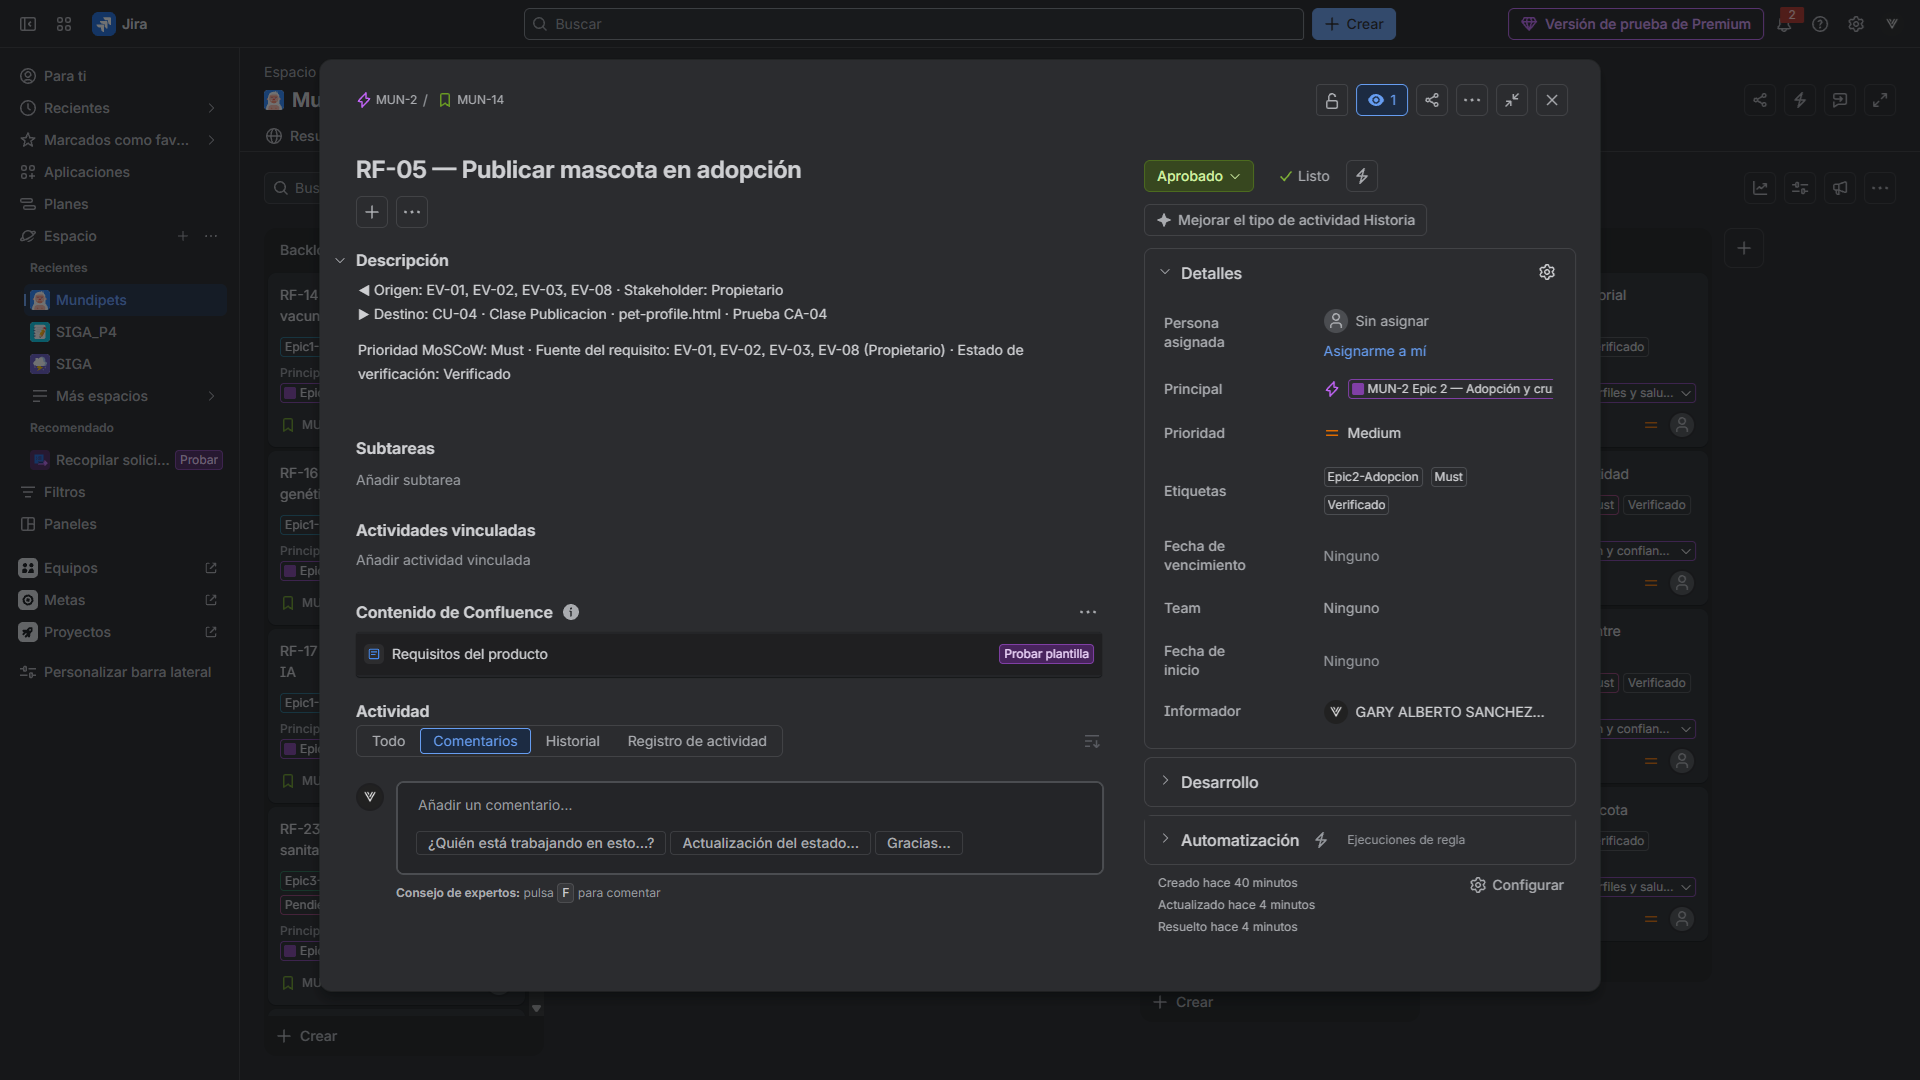
\includegraphics[width=0.85\textwidth]{figuras/2026-08-09_jira_RF-05-publicar-mascota-en-adopcion.png}
		\caption{Detalle de issues 1 con campos personalizados y trazabilidad.}
		\label{fig:tarjetas-detalle1}
	\end{figure}
	
	\begin{figure}[H]
		\centering
		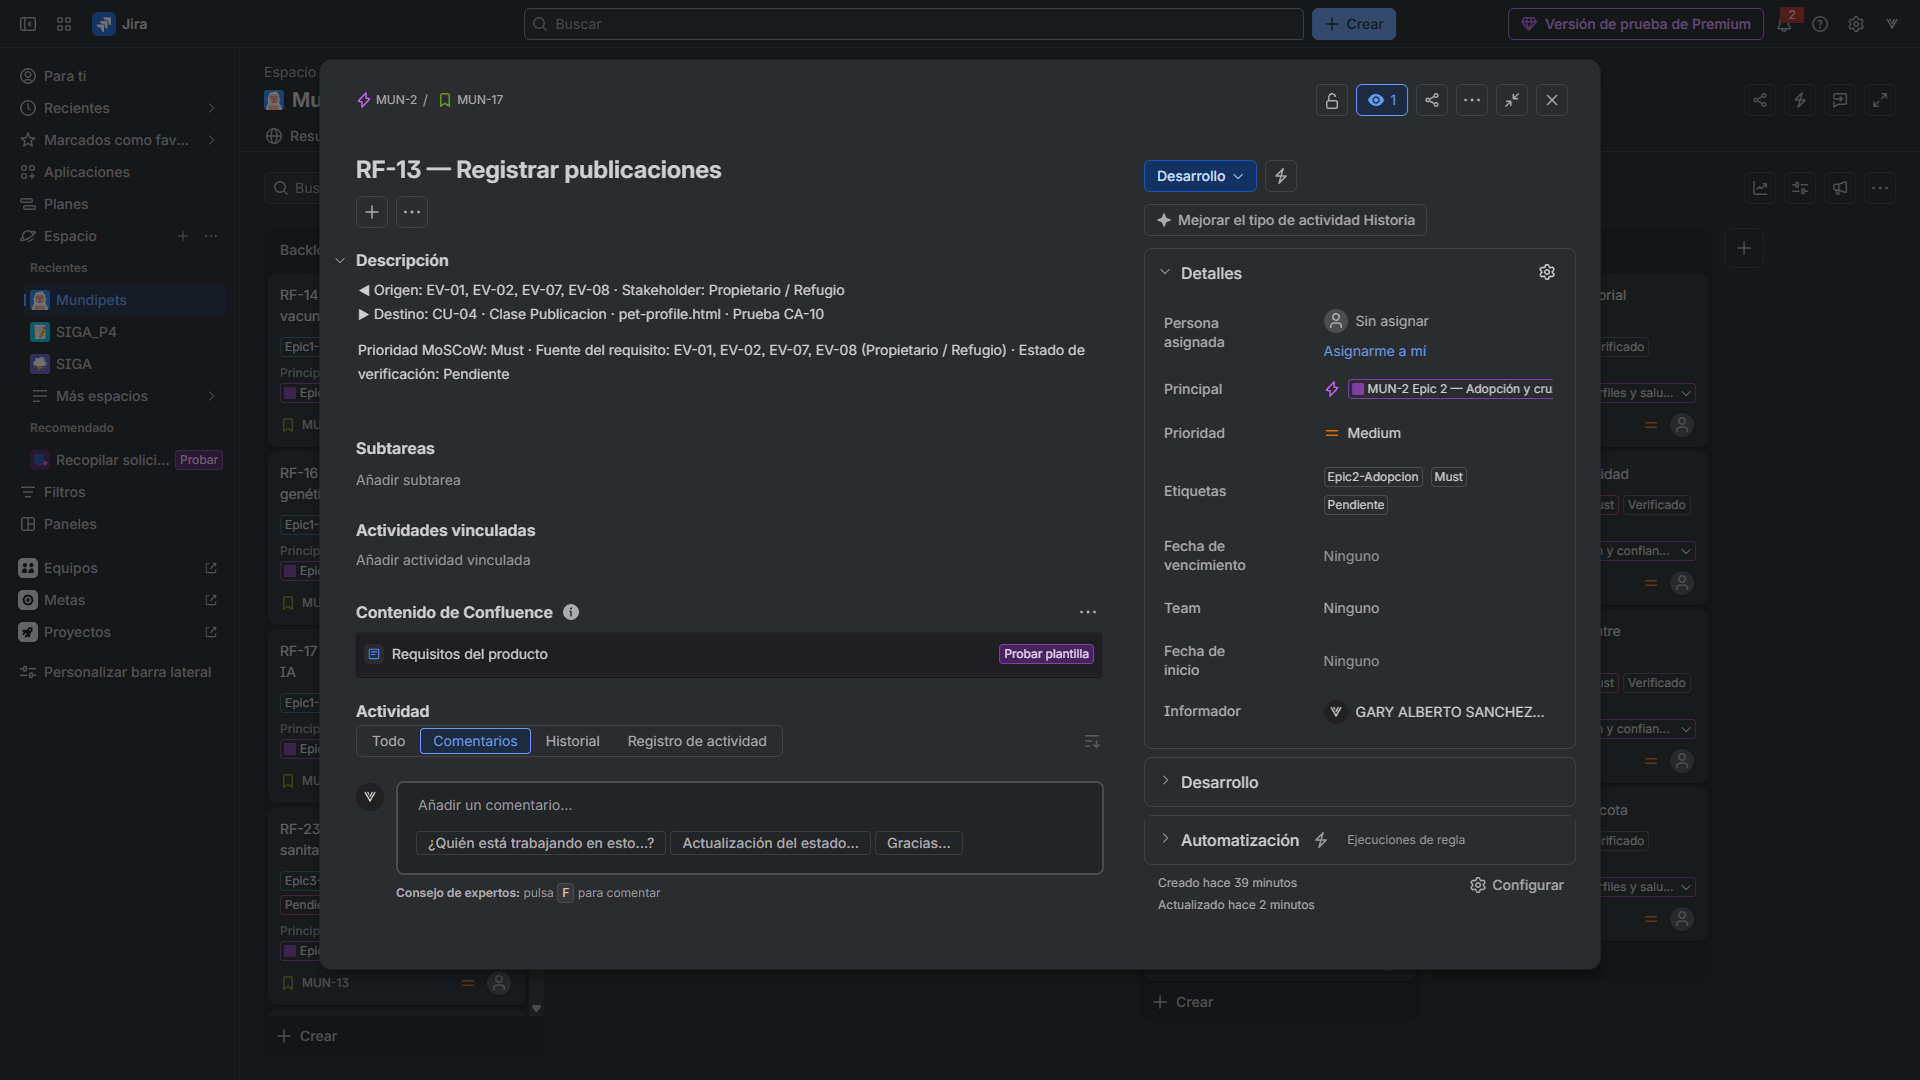
\includegraphics[width=0.85\textwidth]{figuras/2026-08-09_jira_RF-13-registrar-publicaciones.png}
		\caption{Detalle de issues 2 con campos personalizados y trazabilidad.}
		\label{fig:tarjetas-detalle2}
	\end{figure}
	
		\begin{figure}[H]
		\centering
		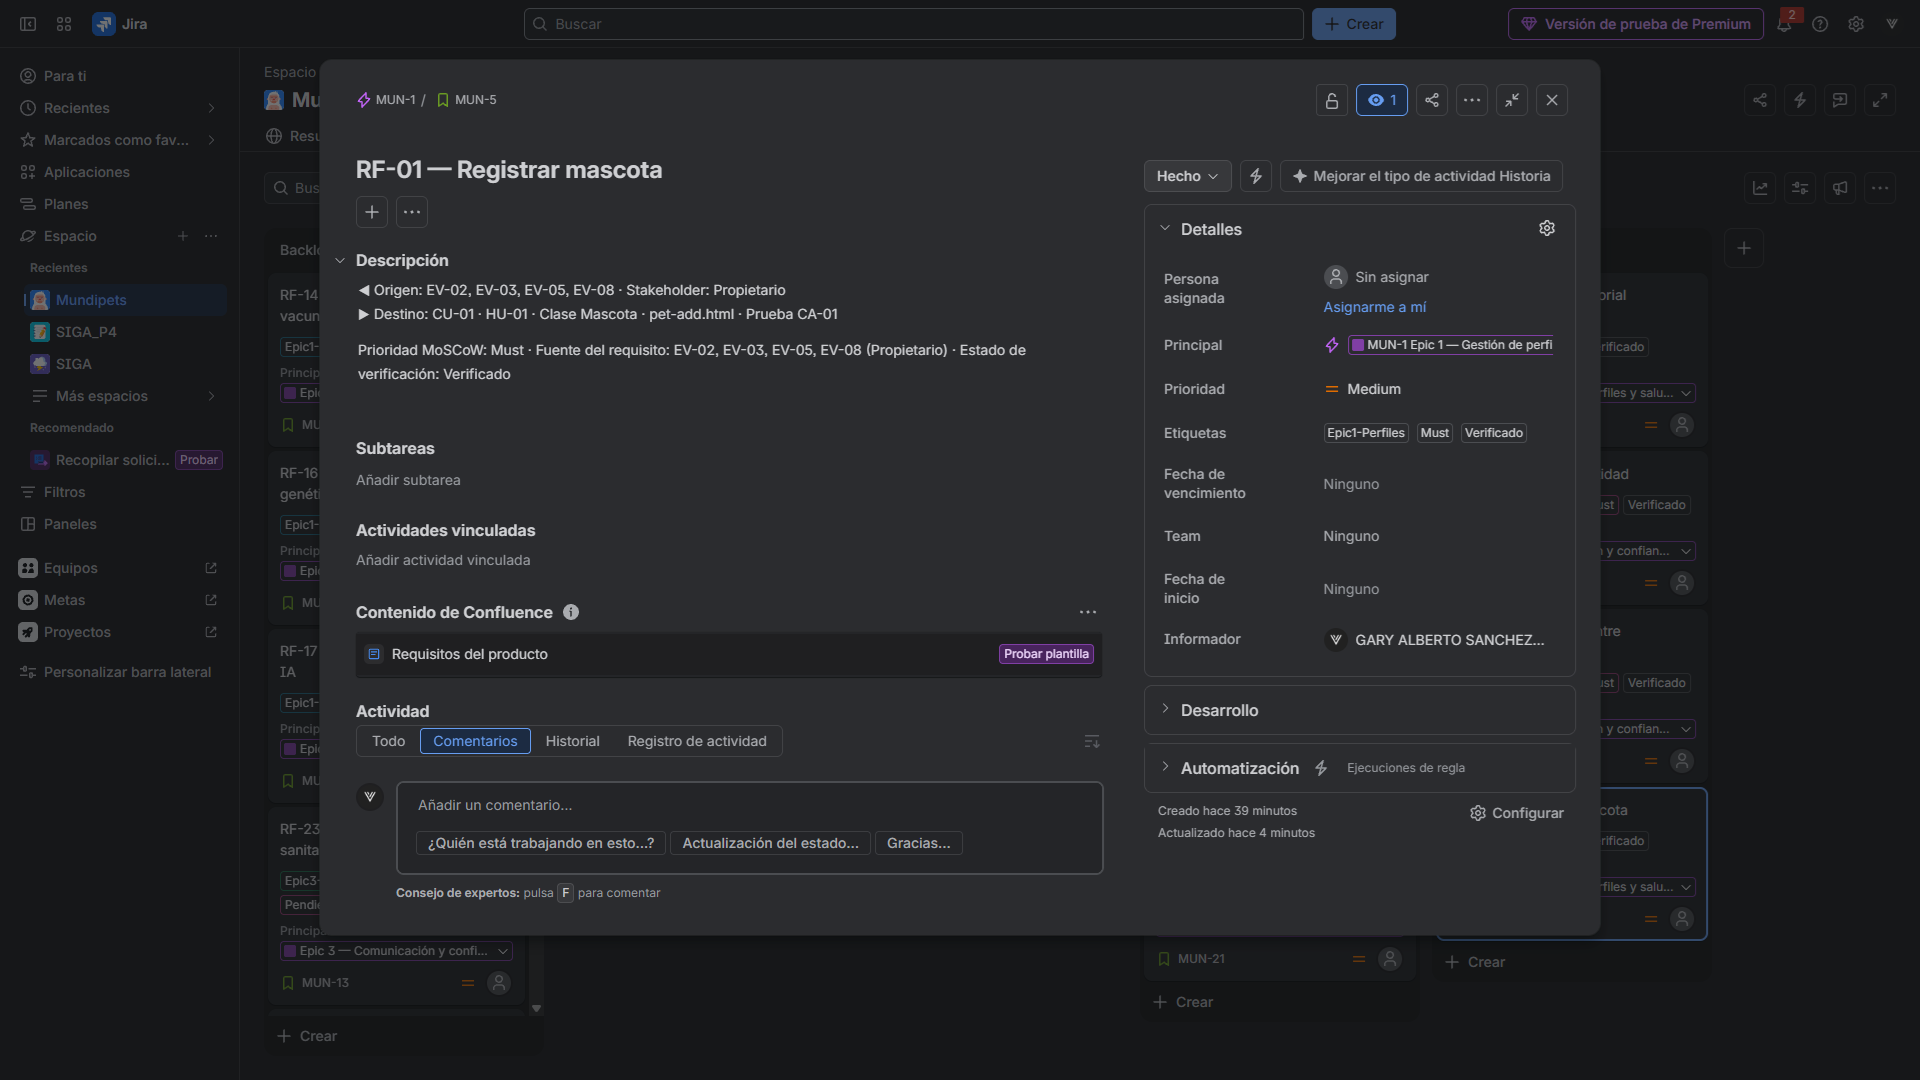
\includegraphics[width=0.85\textwidth]{figuras/2026-08-09_jira_RF-01-registrar-mascota.png}
		\caption{Detalle de issues 3 con campos personalizados y trazabilidad.}
		\label{fig:tarjetas-detalle3}
	\end{figure}

	
	\begin{figure}[H]
		\centering
		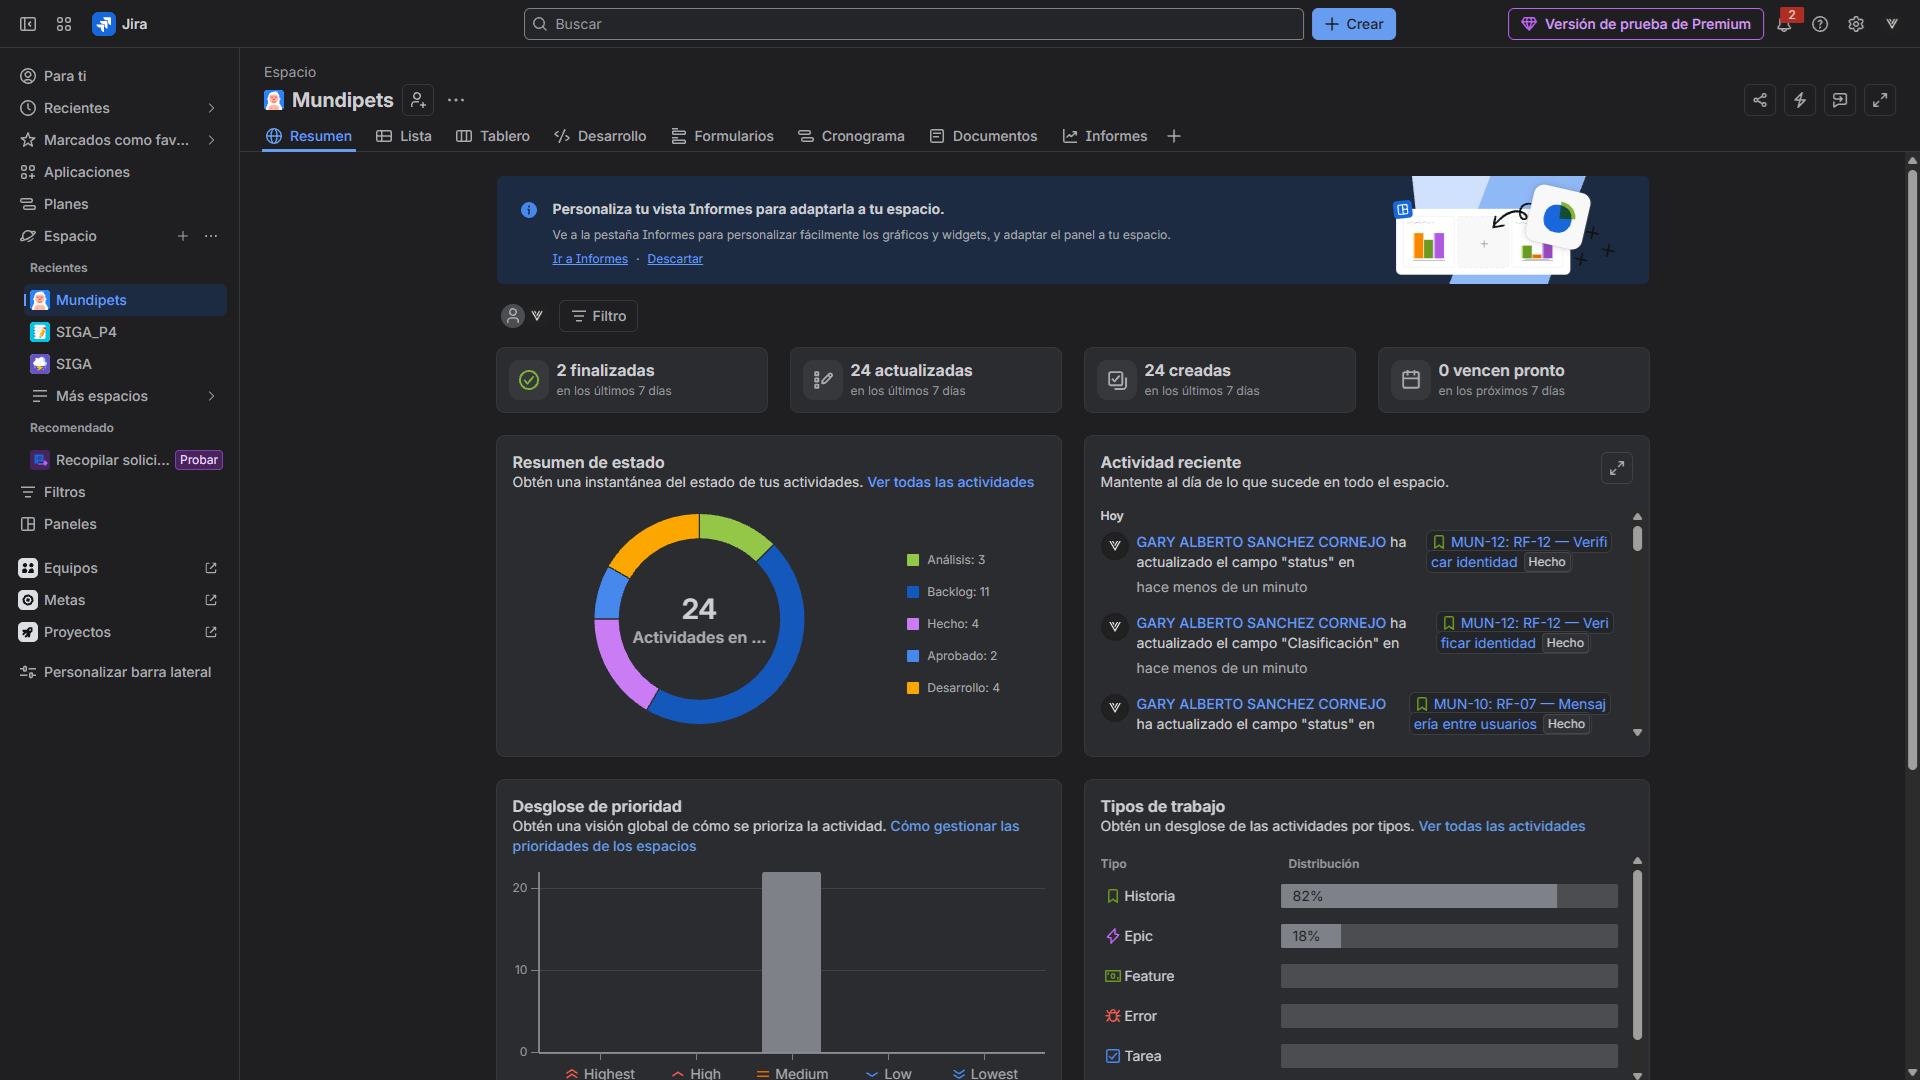
\includegraphics[width=0.85\textwidth]{figuras/2026-08-09_jira_resumen.png}
		\caption{Panel de resumen del proyecto CASE en Jira.}
		\label{fig:panel-estadisticas}
	\end{figure}
	
	\begin{figure}[H]
		\centering
		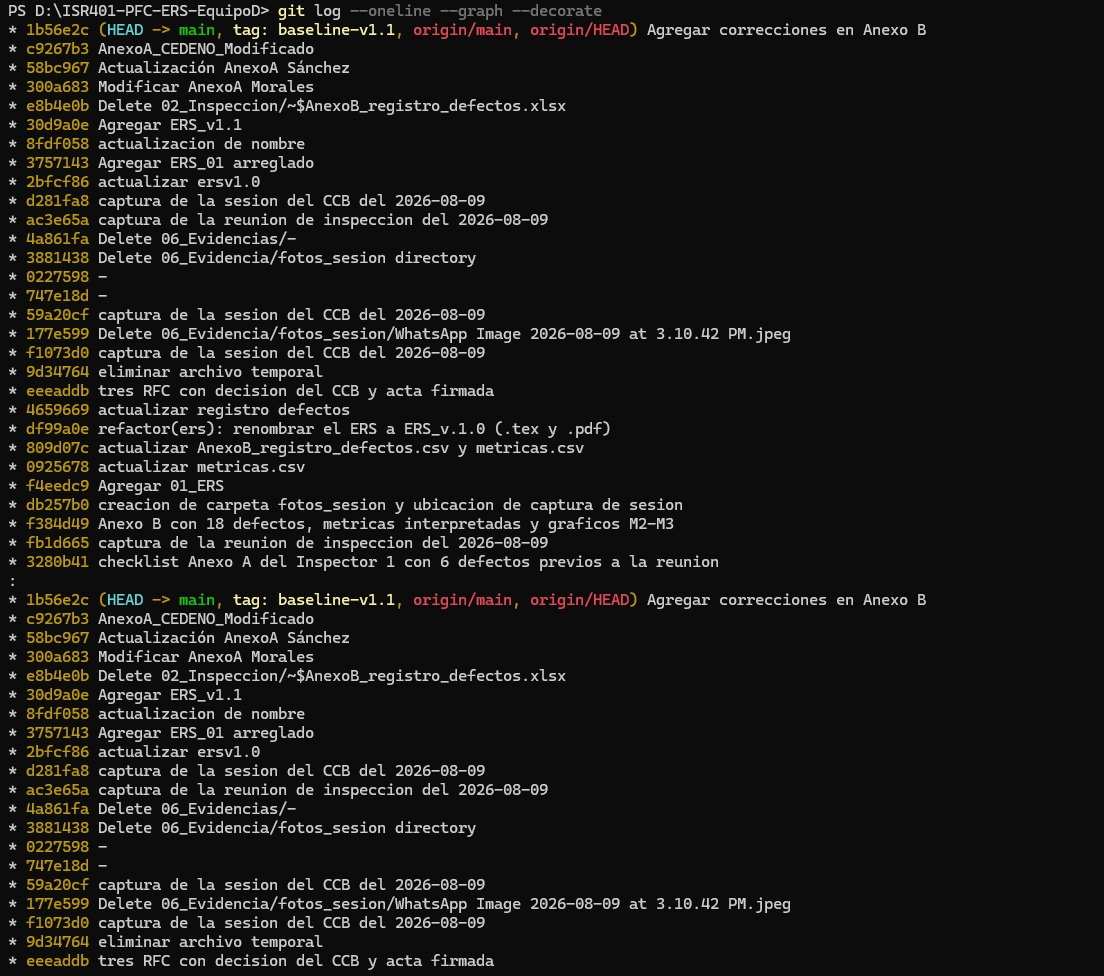
\includegraphics[width=0.85\textwidth]{figuras/gitlogonline.jpeg}
		\caption{Historial de commits (\texttt{git log --oneline --graph --decorate}).}
		\label{fig:git-log}
	\end{figure}
	
	\begin{figure}[H]
		\centering
		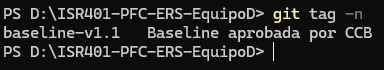
\includegraphics[width=0.6\textwidth]{figuras/gittag.jpeg}
		\caption{Etiqueta de línea base publicada (\texttt{git tag -n}), \texttt{baseline-v1.1}.}
		\label{fig:git-tag}
	\end{figure}
	
	\subsection*{Historial de commits en GitHub (evidencia adicional)}
	
	\begin{figure}[H]
		\centering
		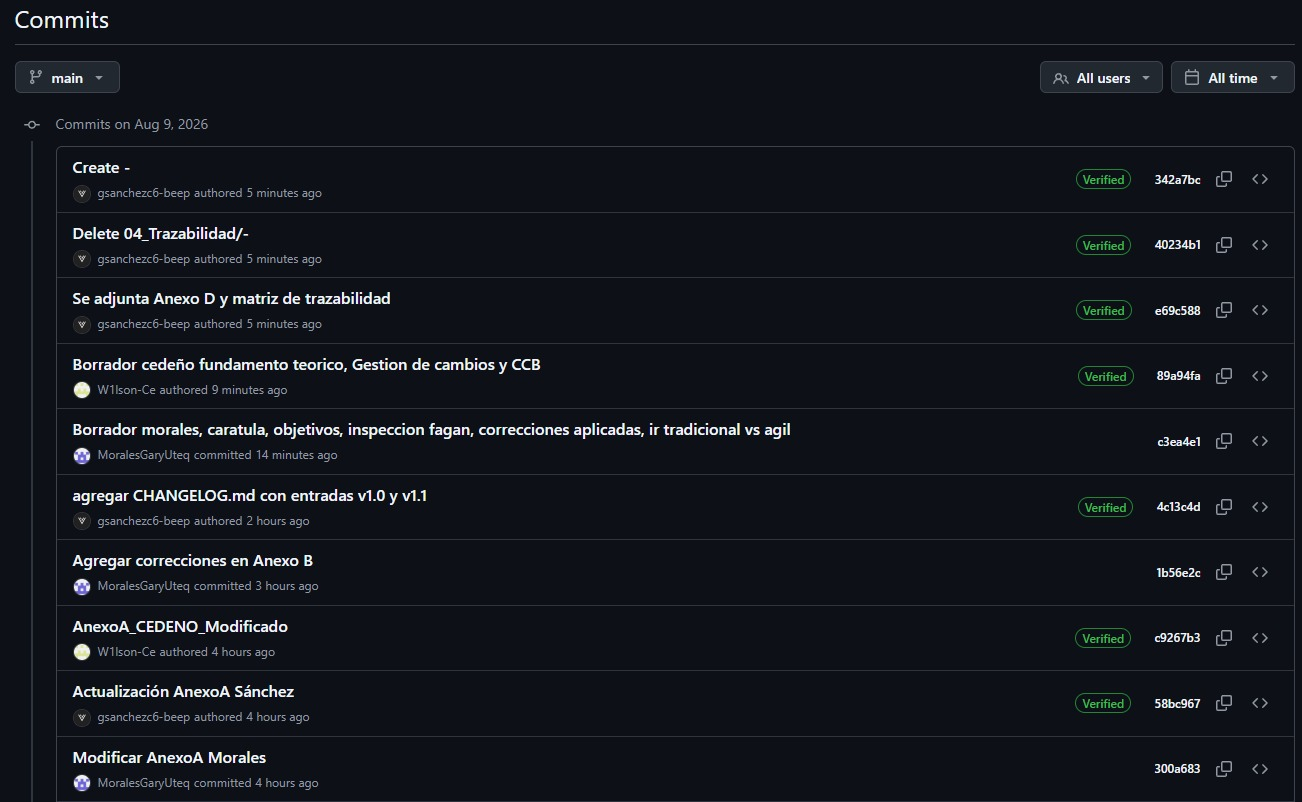
\includegraphics[width=0.85\textwidth]{figuras/evidenciagit1.jpeg}
		\caption{Vista del repositorio en GitHub con los commits más recientes.}
		\label{fig:evidencia-git-1}
	\end{figure}
	
	\begin{figure}[H]
		\centering
		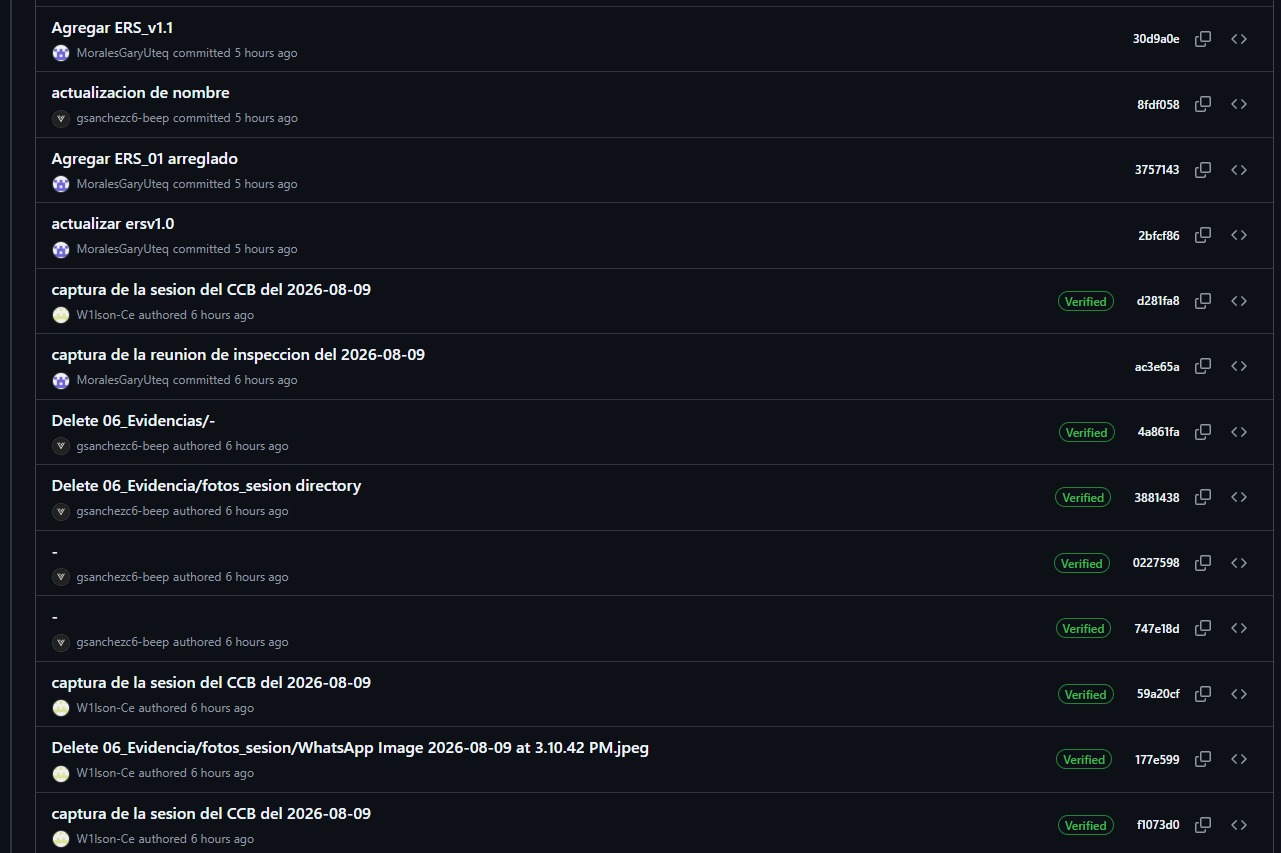
\includegraphics[width=0.85\textwidth]{figuras/evidenciagit2.jpeg}
		\caption{Continuación del historial de commits en GitHub, con autoría distribuida entre los tres integrantes del equipo.}
		\label{fig:evidencia-git-2}
	\end{figure}
	
	\section{Referencias IEEE y declaración de uso de IA}
	\label{ap:anexoF}
	
	\subsection*{F.1 Referencias adicionales citadas en este anexo}
	
	\printbibliography[title={Referencias}]
	
	\subsection*{F.2 Declaración de uso de inteligencia artificial}
	
	\begin{atributos}{declaracion-ia}{Declaración de uso de IA generativa (Anexo F).}
		Herramienta y versión & Claude (Anthropic), modelo Claude Sonnet 4.5, acceso vía interfaz de chat \\
		Tarea asistida & Apoyo en la redacción y estructuración de los formularios RFC, el acta del CCB y la maquetación \LaTeX{} del informe, a partir de los defectos, decisiones y datos provistos directamente por el equipo \\
		Fragmento afectado & Secciones 6 (Gestión del cambio y CCB), 7 (Trazabilidad), 9 (Comparativa CASE) y los Anexos C y D \\
		Verificación crítica realizada por el equipo & Cada RFC, decisión del CCB, fila de la matriz de trazabilidad y cifra de las métricas de inspección fue contrastada por el equipo contra el ERS real, el tablero CASE y el repositorio Git antes de incorporarse al informe final; ningún dato numérico ni referencia bibliográfica se incorporó sin verificación directa contra su fuente \\
		Firma de los integrantes & \parbox[t]{11.2cm}{
			Morales Sánchez: \raisebox{-0.7\height}{
\includegraphics[height=1.0cm]{figuras/firmaMorales.jpeg}} \\[4pt]
			Sánchez Cornejo: \raisebox{-0.7\height}{
\includegraphics[height=1.0cm]{figuras/firmaSanchez.jpeg}} \\[4pt]
			Cedeño Coronado: \raisebox{-0.7\height}{
\includegraphics[height=1.0cm]{figuras/firmaCedeno.jpeg}}
		} \\
	\end{atributos}
	
\end{document}